\chapter{Experimental Results} \label{ch:ExperimentalResults}
In this Chapter we will cover the experimental phase of our work. First comes a description of our setup and methodology, covering the hardware and software utilized as well as the chosen benchmarks and metrics. Then we will present our results and provide our analysis in order to fuel further research and development in the MANGO software stack.

During this experimental campaign, our goals were to:
\begin{itemize}
    \item Compare MANGO with other available programming models, in terms of performance and programmability.
    \item Analyze where the main overheads of the current MANGO implementation are and how they can be reduced.
    \item Evaluate our communication scheme between the Libmango API and the HHAL client, and how it can be improved.
\end{itemize}

\section{Setup and Methodology} \label{sect:setup-methodology}
All our tests were run on a Dell XPS 9570 laptop. This particular model is equipped with an Intel Core i7 8750H CPU, 16 GB RAM and an Nvidia GeForce GTX 1050 Ti GPU with Max-Q Design (4GB VRAM). In terms of Operating System, the machine was running Ubuntu 18.04.2 LTS 64-bit (Kernel Version: 5.4.0-48-generic).

For reproducibility, the versions of the software run were the following:
\begin{itemize}
    \item CUDA 11.0
    \item OpenCL 1.2 CUDA (Driver version: 450.51.06)
    \item gcc 7.5.0 (Ubuntu 7.5.0-3ubuntu1~18.04)
    \item clang 6.0.0-1ubuntu2
    \item Python 3.6.9
    \item Cython 0.29.23
\end{itemize}

In order to compare the performance of MANGO to CUDA and OpenCL we used a subset of the Rodinia Benchmark Suite (Version 3.1) \cite{rodinia}, provided by the University of Virginia. In particular, we chose the HotSpot and PathFinder benchmarks.

HotSpot (HS) is a thermal simulation tool, presented in \cite{hotspot}, which is used for estimating processor temperature based on an architectural floor plan and simulated power measurements. The benchmark includes the 2D transient thermal simulation kernel of HotSpot, which iteratively solves a series of differential equations for block temperatures. The inputs to the program are power and initial temperatures of a square N x N grid. Each output cell in the grid represents the average temperature value of the corresponding area of the chip.

During our experiments, the size of the Grid (N) was progressively increased in order to increase the load on the GPU. The number of threads spawned for computation as well as the size of the input buffers and output buffers scale with O(N\textsuperscript{2}). The number of kernel executions is determined by the amount of iterations desired. This parameter is kept fixed, resulting in 16 kernel executions to compute 128 iterations of the algorithm for all HotSpot benchmarks.

PathFinder (PF) uses dynamic programming to find a path on a 2-D grid from the bottom row to the top row with the smallest accumulated weights, where each step of the path moves straight ahead or diagonally ahead. It iterates row by row, each node picks a neighboring node in the previous row that has the smallest accumulated weight, and adds its own weight to the sum.

Like with HotSpot, we also increased the size of the input grid (N) in order to increase the GPU load when running the PathFinder benchmarks. The dimensions of the grid were also kept symmetrical, as in the number of columns is equal to the number of rows (N x N). In this case, increasing the number of columns increases the number of threads spawn to compute the shortest path. The number of rows, on the other hand, increases the number of kernel executions. In addition, the size of the grid increases the dimensions of the input buffer with O(N\textsuperscript{2}), the output however only increases linearly, with O(N), as only the values of the columns are needed.

During our testing we realized that PathFinder most certainly lacks global GPU memory access optimizations. This is indicated by its poor memory bandwidth performance coupled with the fact that the algorithm requires continuous access to the input rows in order to calculate each iteration. In addition, the operations performed by pathfinder are simple comparisons and a single integer addition. It is important to also note that these comparisons are integer minimum operations, which do not generate branches \cite{ptx_isa}.

We still decided to keep PathFinder in our comparison as it is a good example of what happens when there is a need to run a kernel multiple times in a single benchmark and how the different systems scale with increasing numbers of kernel launches.

Finally, in order to cover our lack of memory bound applications due to the issues mentioned with PathFinder, we added an AXPY benchmark. AXPY stands for "A X plus Y", as noted by the name, it performs the following operation:

\[
    z \leftarrow a*x+y
\]

This same operation is also implemented in BabelStream \cite{babelstream}, a memory bandwidth benchmark for heterogenous systems based on STREAM \cite{stream}, which names it "Triad". 

A breakdown of the three benchmarks chosen can be seen in table \ref{tab:benchmark-breakdown}.

\begin{table}[ht]
    \centering
    \begin{tabular}{l|c|c}
    Benchmark & Dwarves & Performance characteristic \\ \hline
    HotSpot & Structured Grid & Compute intensive \\
    PathFinder & Dynamic Programming & Multiple kernel launches \\
    AXPY & Basic Linear Algebra & Memory intensive          
    \end{tabular}
    \captionsetup{justification=centering}
    \caption{Breakdown of benchmarks used}
    \label{tab:benchmark-breakdown}
\end{table}

\subsection{Performance metrics}

To evaluate performance in both HotSpot and PathFinder, we will measure:

\begin{itemize}
    \item Total execution time: Time since the beginning of the proper benchmark (i.e. after all input initialization and I/O) and the end (after all resource deallocations, but before checking output results).
    \item Kernel execution time: Time since the launch of a kernel and the end of its execution.
    \item Buffer write time: Time to write data to the device, i.e transfer data from the host to the device.
    \item Buffer read time: Time to read data from the device, i.e. transfer data from the device to the host.
\end{itemize}

For AXPY, we will measure the performance of the different systems as the percentage of theoretical peak bandwidth they can achieve. We will take into account both GPU memory bandwidth, measuring accesses to GPU global memory, and PCI-E bandwidth, measuring data transfers between the Host and the Device and vice versa.

For GPU memory, the theoretical peak bandwidth is given by plugging the memory clock rate and bus width into the following formula:

\[
    GBW_{peak} = \frac{C * 10^6 * (B/8) * 2}{10^9}
\]

Where:
\begin{itemize}
    \item $GBW_{peak}$ is the theoretical peak GPU VRAM bandwidth in GB/s.
    \item $C$ is the memory clock rate in MHz.
    \item $B$ is the memory bus width in bits.
\end{itemize}

With a memory clock rate of 3504 MHz and 128-bit of bus width, the GTX 1050 Ti in our test bench achieves a theoretical peak of 112.128 GB/s.

To measure the effective bandwidth achieved by each model we use the following formula:

\[
    GBW_{effective} = \frac{R_B + W_B}{t * 10^9}
\]

Where:
\begin{itemize}
    \item $GBW_{effective}$ is the effective GPU VRAM bandwidth in GB/s.
    \item $R_B$ is the number of bytes read per kernel.
    \item $W_B$ is the number of bytes written per kernel.
    \item $t$ is the kernel execution time in seconds.
\end{itemize}

The two previous formulae were taken from \cite{perf_metrics_cuda}.

In terms of PCI-E bandwidth, our video card presents a PCI-E 3.0 x16 connection which could achieve a peak bandwidth of 15.754GB/s.

In a very similar way as how we measure effective bandwidth for GPU memory, we can measure the effective transfer bandwidth:

\[
    TBW_{effective} = \frac{T_B}{t * 10^9}
\]

Where:
\begin{itemize}
    \item $TBW_{effective}$ is the effective transfer bandwidth in GB/s.
    \item $T_B$ is the number of bytes transferred.
    \item $t$ is the transfer time in seconds.
\end{itemize}

In AXPY we are not interested in the scaling over different input sizes but in the bandwidths achieved with large inputs. A large input maximizes the amount of memory to transfer and access, meaning that a larger part of the available bandwidth can be exploited.

It is important to note that for all benchmarks in both CUDA and OpenCL we execute the set of benchmarks twice. Once to measure the total execution time of the entire benchmark and another to measure each individual component. As all our measurements in these models are done externally (i.e. we cannot make intrusive profiling modifications like with MANGO) they could incur in extra overhead due to the need of forcing synchronization between the host and the device in order to make measurements. For example, OpenCL buffer writes are usually enqueued in a \texttt{CommandQueue} and executed asynchronously, to measure them we forced a synchronous transfer by calling \texttt{clFinish} on the \texttt{CommandQueue}.

In the case of MANGO, to evaluate its performance and compare it directly with CUDA and OpenCL we perform profiling of the application at the HHAL server, disregarding the overhead added by IPC communication. As mentioned previously, the HHAL library is implemented in a client-server arrangement, where the communication between client and server is performed via a socket. This provides us with an easy way to run the HHAL in a separate cluster in the future. However, it adds extra communication overhead to the MANGO client which is not present in either CUDA nor OpenCL, as they both are designed to run directly on the same host machine as the target accelerator.

\subsection{IPC}
To evaluate the communication scheme between Libmango and HHAL, we also performed measurements directly on the Libmango API side. This measurements will also take the previously mentioned IPC overhead into account, which we will compare directly with the metrics obtained on the HHAL server itself. The discrepancies between the two sets of values will provide us with an overview of the aspects of the system that are most affected by IPC communication and how they could be improved.

\subsection{Programmability}

To compare the programmability of each model we count the number of lines of code (LOC) required for each implementation of the HotSpot and PathFinder benchmarks. To compute the LOC we do not take into account comments or blank lines. Also, we ignore any line of code related to debugging, extra code needed to profile the OpenCL and CUDA benchmarks or checking computation results. This last point is particularly significant on the MANGO benchmarks which usually compare their results with the CUDA benchmarks to ensure that the implementation is working correctly. Finally, the original code from the Rodinia Benchmarks was adapted in order to follow a consistent style across all implementations. 

In addition to the LOC metric, to have a more direct comparison of the size of the MANGO implementations to the CUDA and OpenCL ones we also use a Relative Difference metric (RD). RD calculates the percentage difference in LOC between MANGO and a different implementation. We define RD as follows:

\[
    RD = \frac{LOC_{impl} - LOC_{MANGO}}{LOC_{MANGO}} * 100
\]

Thus, a positive RD indicates that a given implementation requires more LOC than MANGO, while a negative RD indicates that the implementation requires less LOC.

\section{Results}

In this section we will present the results of our experiments. First, we will make performance comparisons against CUDA and OpenCL, then we will cover the overhead experimented by the client due to IPC with the HHAL server. Finally, we will analyze the programmability improvements achieved by MANGO over CUDA and OpenCL.

\subsection{Performance}

\subsubsection{HotSpot}

Starting with HotSpot, we can see that performance across all metrics is very similar for all of the different programming model implementations. In addition, all models follow the same scaling as input size increases. 

The overhead presented by MANGO in this benchmark is noticeable, but not significant. For example, when running with a grid size of 8192 x 8192, CUDA is the fastest completing the entire execution in \textasciitilde 2516ms while MANGO takes \textasciitilde 2692ms, a difference of only 6.5\%. 

\begin{figure}
    \centering
    \resizebox{!}{180pt}{
        % This file was created by tikzplotlib v0.9.8.
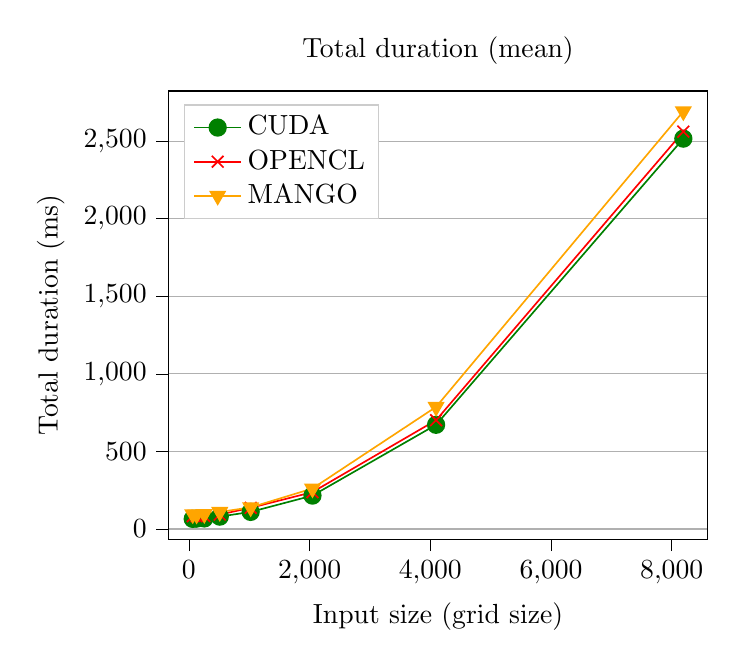
\begin{tikzpicture}

\definecolor{color0}{rgb}{1,0.647058823529412,0}

\begin{axis}[
legend cell align={left},
legend style={
  fill opacity=1,
  draw opacity=1,
  text opacity=1,
  at={(0.03,0.97)},
  anchor=north west,
  draw=white!80!black
},
tick align=outside,
tick pos=left,
title={Total duration (mean)},
x grid style={white!69.0196078431373!black},
xlabel={Input size (grid size)},
xmin=-342.4, xmax=8598.4,
xtick style={color=black},
y grid style={white!69.0196078431373!black},
ylabel={Total duration (ms)},
ymajorgrids,
ymin=-65.959002829394, ymax=2823.53145097283,
ytick style={color=black}
]
\addplot [semithick, green!50.1960784313725!black, mark=*, mark size=3, mark options={solid}]
table {%
64 65.3814723434343
128 67.1212662244898
256 68.3322663666667
512 80.0275030333333
1024 110.4768081
2048 215.540796947368
4096 671.9512696
8192 2516.1915956
};
\addlegendentry{CUDA}
\addplot [semithick, red, mark=x, mark size=3, mark options={solid}]
table {%
64 82.7704575208333
128 82.79732128
256 83.8056829333333
512 93.437536862069
1024 136.60162595
2048 237.940542842105
4096 701.5180952
8192 2561.3243602
};
\addlegendentry{OPENCL}
\addplot [semithick, color0, mark=triangle*, mark size=3, mark options={solid,rotate=180}]
table {%
64 95.13603588
128 93.41098096
256 96.4721031
512 110.236007833333
1024 139.4998439
2048 261.1760106
4096 787.2880039
8192 2692.1909758
};
\addlegendentry{MANGO}
\end{axis}

\end{tikzpicture}

    }
    \captionsetup{justification=centering}
    \caption{Mean total execution time for HotSpot}
    \label{fig:hotspot_total_duration_mean}
\end{figure}

When decomposing the benchmark into its different aspects we can see that the overhead is most significant for buffer writes, as seen in figure \ref{fig:hotspot_buffer_transfers_mean}. Here CUDA is 8.4\% faster than MANGO for the same 256 megabyte transfer. Still, MANGO keeps up the pace with OpenCL, which is only 1\% faster.

\begin{figure}%
    \centering
    \subfloat[\centering Mean buffer write time]{{
        \resizebox{!}{160pt}{
        % This file was created by tikzplotlib v0.9.8.
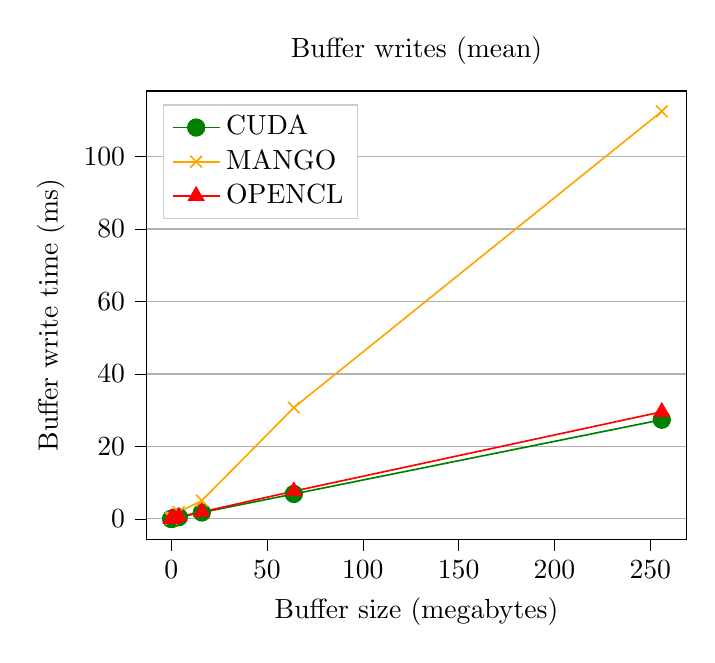
\begin{tikzpicture}

\definecolor{color0}{rgb}{1,0.647058823529412,0}

\begin{axis}[
legend cell align={left},
legend style={
  fill opacity=1,
  draw opacity=1,
  text opacity=1,
  at={(0.03,0.97)},
  anchor=north west,
  draw=white!80!black
},
tick align=outside,
tick pos=left,
title={Buffer writes (mean)},
x grid style={white!69.0196078431373!black},
xlabel={Buffer size (megabytes)},
xmin=-12.78359375, xmax=268.79921875,
xtick style={color=black},
y grid style={white!69.0196078431373!black},
ylabel={Buffer write time (ms)},
ymajorgrids,
ymin=-5.6126042730303, ymax=118.094086289192,
ytick style={color=black},
yticklabel style={/pgf/number format/fixed},
]
\addplot [semithick, green!50.1960784313725!black, mark=*, mark size=3, mark options={solid}]
table {%
0.015625 0.0104271161616162
0.0625 0.0190681313131313
0.25 0.0421460666666667
1 0.138006
4 0.479187025
16 1.777260975
64 6.89048626315789
256 27.3749119473684
};
\addlegendentry{CUDA}
\addplot [semithick, color0, mark=x, mark size=3, mark options={solid}]
table {%
0.015625 0.132945717948718
0.0625 0.1841103
0.25 0.203108508474576
1 0.371122457627119
4 1.873227375
16 5.05497213157895
64 30.71298635
256 112.4710549
};
\addlegendentry{MANGO}
\addplot [semithick, red, mark=triangle*, mark size=3, mark options={solid}]
table {%
0.015625 0.0693875846153846
0.0625 0.0795439081632653
0.25 0.1081564
1 0.245969101694915
4 0.625349487179487
16 1.934185
64 7.6582627
256 29.54956935
};
\addlegendentry{OPENCL}
\end{axis}

\end{tikzpicture}

    } 
    }}%
    \qquad
    \subfloat[\centering Mean buffer read time]{{
        \resizebox{!}{160pt}{
            % This file was created by tikzplotlib v0.9.8.
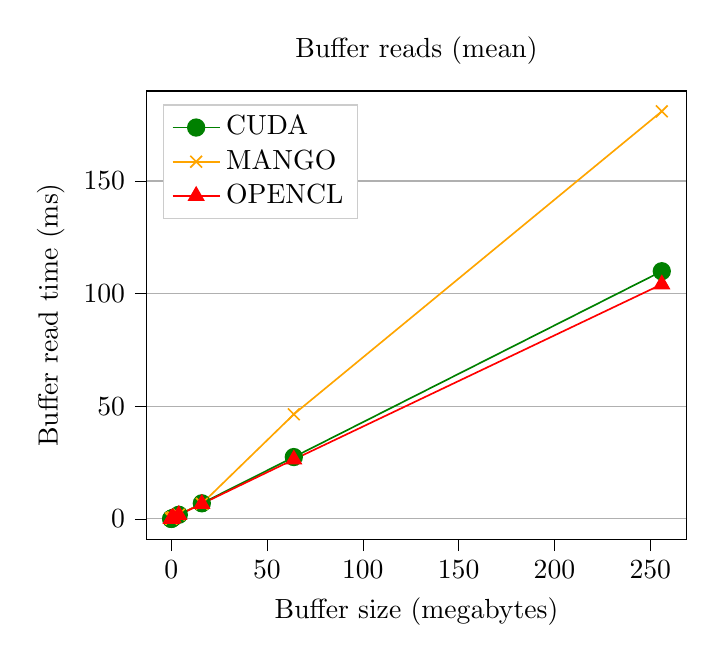
\begin{tikzpicture}

\definecolor{color0}{rgb}{1,0.647058823529412,0}

\begin{axis}[
legend cell align={left},
legend style={
  fill opacity=1,
  draw opacity=1,
  text opacity=1,
  at={(0.03,0.97)},
  anchor=north west,
  draw=white!80!black
},
tick align=outside,
tick pos=left,
title={Buffer reads (mean)},
x grid style={white!69.0196078431373!black},
xlabel={Buffer size (megabytes)},
xmin=-12.78359375, xmax=268.79921875,
xtick style={color=black},
y grid style={white!69.0196078431373!black},
ylabel={Buffer read time (ms)},
ymajorgrids,
ymin=-9.03422905142857, ymax=189.990061773878,
ytick style={color=black},
yticklabel style={/pgf/number format/fixed},
]
\addplot [semithick, green!50.1960784313725!black, mark=*, mark size=3, mark options={solid}]
table {%
0.015625 0.0123296224489796
0.0625 0.0205413469387755
0.25 0.130403275862069
1 0.505512620689655
4 1.83742425
16 6.9285274
64 27.4589087
256 109.953671
};
\addlegendentry{CUDA}
\addplot [semithick, color0, mark=x, mark size=3, mark options={solid}]
table {%
0.015625 0.0806020101010101
0.0625 0.16509962
0.25 0.282117206896552
1 0.732995033333333
4 1.89954115
16 6.7418782
64 46.451228
256 180.9435031
};
\addlegendentry{MANGO}
\addplot [semithick, red, mark=triangle*, mark size=3, mark options={solid}]
table {%
0.015625 0.0137764387755102
0.0625 0.02193194
0.25 0.136782633333333
1 0.511125655172414
4 1.78901245
16 6.68551331578947
64 26.398961
256 104.1510284
};
\addlegendentry{OPENCL}
\end{axis}

\end{tikzpicture}

        } 
    }}%
    \captionsetup{justification=centering}
    \caption{Mean buffer transfer times for HotSpot}%
    \label{fig:hotspot_buffer_transfers_mean}%
\end{figure}

The most important overhead is actually the one linked to kernel executions, which are performed more frequently than buffer writes (only 2 buffer writes versus 16 kernel executions) and also individually require more time to be performed. In this case, CUDA and OpenCL are 6.2\% and 3.7\% faster respectively for the largest grid size used. This can be seen in figure \ref{fig:hotspot_kernel_executions_mean}.

\begin{figure}
    \centering
    \resizebox{!}{160pt}{
        % This file was created by tikzplotlib v0.9.8.
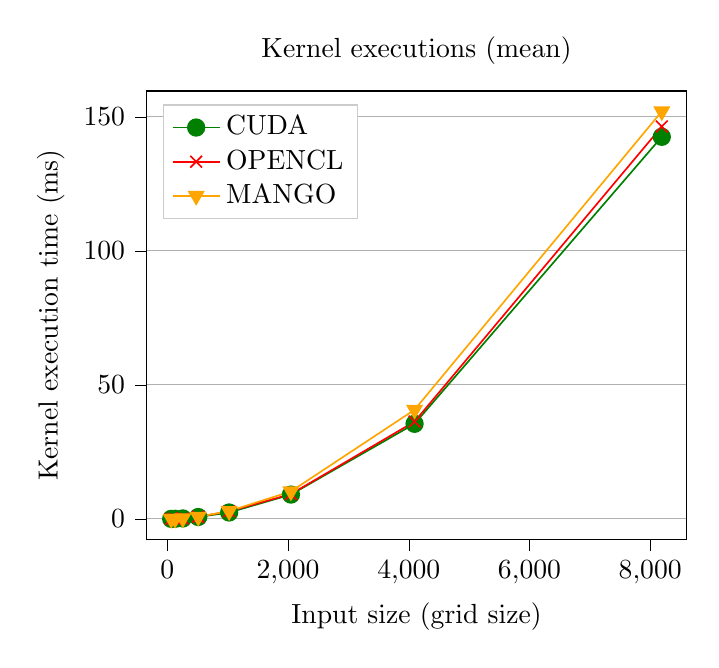
\begin{tikzpicture}

\definecolor{color0}{rgb}{1,0.647058823529412,0}

\begin{axis}[
legend cell align={left},
legend style={
  fill opacity=1,
  draw opacity=1,
  text opacity=1,
  at={(0.03,0.97)},
  anchor=north west,
  draw=white!80!black
},
tick align=outside,
tick pos=left,
title={Kernel executions (mean)},
x grid style={white!69.0196078431373!black},
xlabel={Input size (grid size)},
xmin=-342.4, xmax=8598.4,
xtick style={color=black},
y grid style={white!69.0196078431373!black},
ylabel={Kernel execution time (ms)},
ymajorgrids,
ymin=-7.58184667491691, ymax=159.663488779392,
ytick style={color=black}
]
\addplot [semithick, green!50.1960784313725!black, mark=*, mark size=3, mark options={solid}]
table {%
64 0.0202140275516594
128 0.0516223956466069
256 0.184729111111111
512 0.725393121412804
1024 2.39956375632911
2048 9.09626238291139
4096 35.4947399367089
8192 142.560531045161
};
\addlegendentry{CUDA}
\addplot [semithick, red, mark=x, mark size=3, mark options={solid}]
table {%
64 0.0204119285237141
128 0.0538414779706275
256 0.190541695364238
512 0.780070042826552
1024 2.83085394321767
2048 9.27893204444444
4096 36.3103518152866
8192 146.39821255625
};
\addlegendentry{OPENCL}
\addplot [semithick, color0, mark=triangle*, mark size=3, mark options={solid,rotate=180}]
table {%
64 0.0414139624681934
128 0.0703628888888889
256 0.211658812903226
512 0.81808229004329
1024 2.9290935968254
2048 10.27900955
4096 40.7308336708861
8192 152.061428076923
};
\addlegendentry{MANGO}
\end{axis}

\end{tikzpicture}

    }
    \captionsetup{justification=centering}
    \caption{Mean kernel execution time for HotSpot}
    \label{fig:hotspot_kernel_executions_mean}
\end{figure}

The benchmark breakdown figure \ref{fig:hotspot_breakdown} clearly shows the influence of kernel execution time in the overall running time. This breakdown compares how the total running time of the benchmark is distributed among the different aspects of the execution, plus some miscellaneous operations which are not particularly relevant for this benchmark. To generate these metrics we used the measurements obtained when running the biggest input size for HotSpot, 8192 x 8192. The figure clearly pictures how kernel execution time takes up more than 90\% of the total benchmark time.

\begin{figure}
    \centering
    \resizebox{!}{160pt}{
        % This file was created by tikzplotlib v0.9.8.
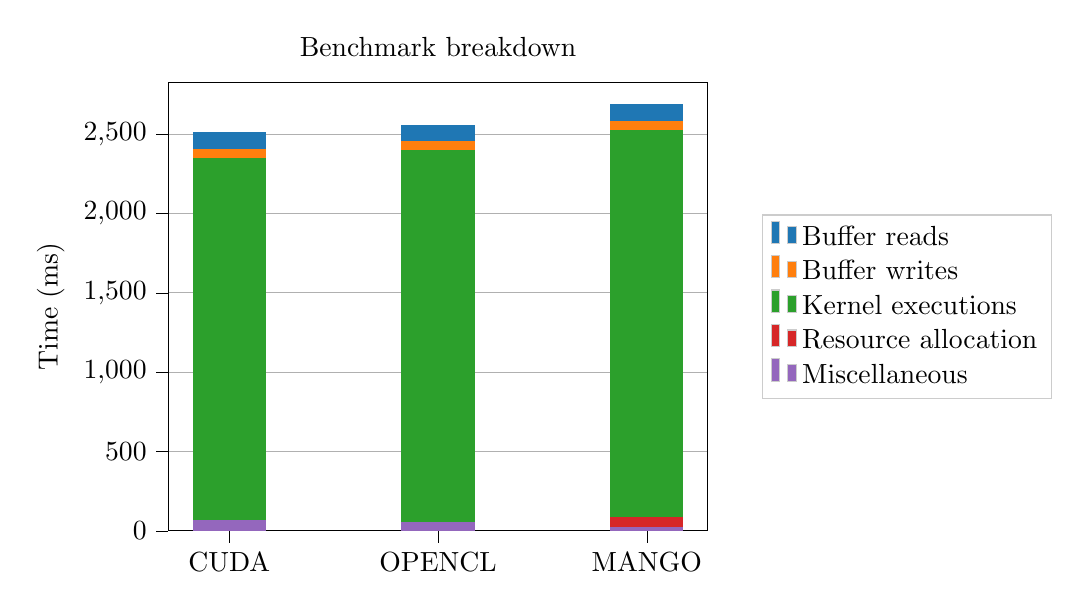
\begin{tikzpicture}

\definecolor{color0}{rgb}{0.12156862745098,0.466666666666667,0.705882352941177}
\definecolor{color1}{rgb}{1,0.498039215686275,0.0549019607843137}
\definecolor{color2}{rgb}{0.172549019607843,0.627450980392157,0.172549019607843}
\definecolor{color3}{rgb}{0.83921568627451,0.152941176470588,0.156862745098039}
\definecolor{color4}{rgb}{0.580392156862745,0.403921568627451,0.741176470588235}

\begin{axis}[
legend cell align={left},
legend style={
  fill opacity=1,
  draw opacity=1,
  text opacity=1,
  at={(1.1,0.5)},
  anchor=west,
  draw=white!80!black
},
tick align=outside,
tick pos=left,
title={Benchmark breakdown},
x grid style={white!69.0196078431373!black},
xmin=-0.2925, xmax=2.2925,
xtick style={color=black},
xtick={0,1,2},
xticklabels={CUDA,OPENCL,MANGO},
y grid style={white!69.0196078431373!black},
ylabel={Time (ms)},
ymajorgrids,
ymin=0, ymax=2826.80052459,
ytick style={color=black}
]
\draw[draw=none,fill=color0] (axis cs:-0.175,2406.2379246) rectangle (axis cs:0.175,2516.1915956);
\draw[draw=none,fill=color0] (axis cs:0.825,2457.1733318) rectangle (axis cs:1.175,2561.3243602);
\draw[draw=none,fill=color0] (axis cs:1.825,2585.467358) rectangle (axis cs:2.175,2692.1909758);
\addlegendimage{ybar,ybar legend,draw=none,fill=color0};
\addlegendentry{Buffer reads}

\draw[draw=none,fill=color1] (axis cs:-0.175,2351.3002211) rectangle (axis cs:0.175,2406.2379246);
\draw[draw=none,fill=color1] (axis cs:0.825,2398.0741931) rectangle (axis cs:1.175,2457.1733318);
\draw[draw=none,fill=color1] (axis cs:1.825,2525.7138286) rectangle (axis cs:2.175,2585.467358);
\addlegendimage{ybar,ybar legend,draw=none,fill=color1};
\addlegendentry{Buffer writes}

\draw[draw=none,fill=color2] (axis cs:-0.175,66.641223) rectangle (axis cs:0.175,2351.3002211);
\draw[draw=none,fill=color2] (axis cs:0.825,55.7027921999998) rectangle (axis cs:1.175,2398.0741931);
\draw[draw=none,fill=color2] (axis cs:1.825,88.8869999000001) rectangle (axis cs:2.175,2525.7138286);
\draw[draw=none,fill=color3] (axis cs:-0.175,66.641223) rectangle (axis cs:0.175,66.641223);
\addlegendimage{ybar,ybar legend,draw=none,fill=color2};
\addlegendentry{Kernel executions}

\draw[draw=none,fill=color3] (axis cs:0.825,55.7027921999998) rectangle (axis cs:1.175,55.7027921999998);
\draw[draw=none,fill=color3] (axis cs:1.825,25.4271799000001) rectangle (axis cs:2.175,88.8869999000001);
\addlegendimage{ybar,ybar legend,draw=none,fill=color3};
\addlegendentry{Resource allocation}

\draw[draw=none,fill=color4] (axis cs:-0.175,0) rectangle (axis cs:0.175,66.641223);
\draw[draw=none,fill=color4] (axis cs:0.825,0) rectangle (axis cs:1.175,55.7027921999998);
\draw[draw=none,fill=color4] (axis cs:1.825,0) rectangle (axis cs:2.175,25.4271799000001);
\addlegendimage{ybar,ybar legend,draw=none,fill=color4};
\addlegendentry{Miscellaneous}

\end{axis}

\end{tikzpicture}

    }
    \captionsetup{justification=centering}
    \caption{Benchmark breakdown for HotSpot}
    \label{fig:hotspot_breakdown}
\end{figure}

\subsubsection{PathFinder}

Moving on to PathFinder we can see a much more significant difference in the performance of MANGO and OpenCL with respect to CUDA in figure \ref{fig:pathfinder_total_duration_mean}. In addition, a clear increase in the steepness of the curve can be seen in the case of MANGO, as it steers away from the OpenCL implementation as the input size increases. This would indicate that there is some noticeable overhead present in the kernel executions, as they increase in number along with the input size of PathFinder.

\begin{figure}
    \centering
    \resizebox{!}{160pt}{
        % This file was created by tikzplotlib v0.9.8.
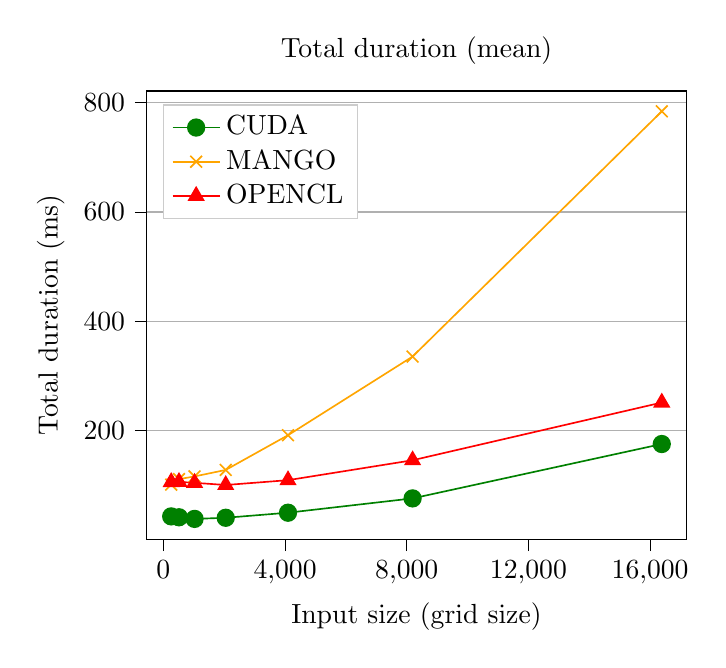
\begin{tikzpicture}

\definecolor{color0}{rgb}{1,0.647058823529412,0}

\begin{axis}[
legend cell align={left},
legend style={
  fill opacity=1,
  draw opacity=1,
  text opacity=1,
  at={(0.03,0.97)},
  anchor=north west,
  draw=white!80!black
},
tick align=outside,
tick pos=left,
title={Total duration (mean)},
x grid style={white!69.0196078431373!black},
xlabel={Input size (grid size)},
xmin=-550.4, xmax=17190.4,
xtick style={color=black},
y grid style={white!69.0196078431373!black},
ylabel={Total duration (ms)},
ymajorgrids,
ymin=1.06305218103449, ymax=821.428003991379,
ytick style={color=black},
scaled x ticks = false,
xtick={0, 4000, 8000, 12000, 16000},
]
\addplot [semithick, green!50.1960784313725!black, mark=*, mark size=3, mark options={solid}]
table {%
256 42.9552711
512 41.32715138
1024 38.3523681724138
2048 40.43792255
4096 49.69510795
8192 75.8983512
16384 175.3781874
};
\addlegendentry{CUDA}
\addplot [semithick, color0, mark=x, mark size=3, mark options={solid}]
table {%
256 101.184211525253
512 111.13555734
1024 116.082388233333
2048 127.939228894737
4096 191.4835014
8192 335.4150991
16384 784.138688
};
\addlegendentry{MANGO}
\addplot [semithick, red, mark=triangle*, mark size=3, mark options={solid}]
table {%
256 105.803828572917
512 106.067160145833
1024 104.400873965517
2048 100.396111
4096 109.2311212
8192 145.6926093
16384 251.2904586
};
\addlegendentry{OPENCL}
\end{axis}

\end{tikzpicture}

    }
    \captionsetup{justification=centering}
    \caption{Mean total execution time for PathFinder}
    \label{fig:pathfinder_total_duration_mean}
\end{figure}

Figure \ref{fig:pathfinder_kernel_executions_mean} confirms our suspicion, as there is a clear separation between the kernel execution times of MANGO and the ones of CUDA and OpenCL, which are quite similar with each other. Comparing the the time taken for the biggest input size, CUDA is 20\% faster than MANGO for each kernel executed, while OpenCL is 17.9\% faster.

\begin{figure}
    \centering
    \resizebox{!}{160pt}{
        % This file was created by tikzplotlib v0.9.8.
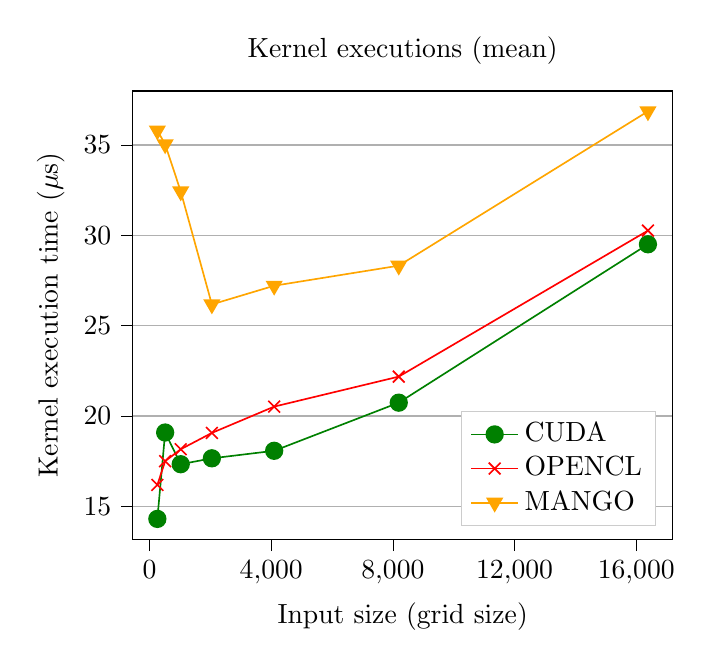
\begin{tikzpicture}

\definecolor{color0}{rgb}{1,0.647058823529412,0}

\begin{axis}[
legend cell align={left},
legend style={
  fill opacity=1,
  draw opacity=1,
  text opacity=1,
  at={(0.97,0.03)},
  anchor=south east,
  draw=white!80!black
},
tick align=outside,
tick pos=left,
title={Kernel executions (mean)},
x grid style={white!69.0196078431373!black},
xlabel={Input size (grid size)},
xmin=-550.4, xmax=17190.4,
xtick style={color=black},
y grid style={white!69.0196078431373!black},
ylabel={Kernel execution time ($\mu$s)},
ymajorgrids,
ymin=13.1755189830914, ymax=37.9917063550803,
ytick style={color=black},
scaled x ticks = false,
xtick={0, 4000, 8000, 12000, 16000},
]
\addplot [semithick, green!50.1960784313725!black, mark=*, mark size=3, mark options={solid}]
table {%
256 14.3035275
512 19.0845953667954
1024 17.3306496732026
2048 17.656685966634
4096 18.0730500490677
8192 20.7366837857667
16384 29.5047277512547
};
\addlegendentry{CUDA}
\addplot [semithick, red, mark=x, mark size=3, mark options={solid}]
table {%
256 16.1839365700861
512 17.4985770416025
1024 18.1579511051574
2048 19.0632247081712
4096 20.5183282178218
8192 22.1790555555556
16384 30.2621266070773
};
\addlegendentry{OPENCL}
\addplot [semithick, color0, mark=triangle*, mark size=3, mark options={solid,rotate=180}]
table {%
256 35.8026210691824
512 35.0376165354331
1024 32.4320626649077
2048 26.175443620178
4096 27.2096125186289
8192 28.3202890760466
16384 36.8636978381717
};
\addlegendentry{MANGO}
\end{axis}

\end{tikzpicture}

    }
    \captionsetup{justification=centering}
    \caption{Mean kernel execution time for PathFinder}
    \label{fig:pathfinder_kernel_executions_mean}
\end{figure}

Focusing now on buffer transfers, as seen in figure \ref{fig:pathfinder_buffer_transfers_mean}, OpenCL gains the advantage for the bigger buffer sizes written by PathFinder. Meanwhile MANGO stays in line with the pure CUDA implementation, although with some overhead still present. In terms of buffer reads, MANGO pulls ahead with the largest buffer size, with CUDA and OpenCL being 28.9\% and 43\% slower respectively. However it is important to note that the buffers read as a result are significantly smaller than the ones written as input, for larger buffer sizes this initial differences could become negligible, as seen for HotSpot in figure \ref{fig:hotspot_buffer_transfers_mean}.

\begin{figure}%
    \centering
    \subfloat[\centering Mean buffer write time]{{
        \resizebox{!}{160pt}{
        % This file was created by tikzplotlib v0.9.8.
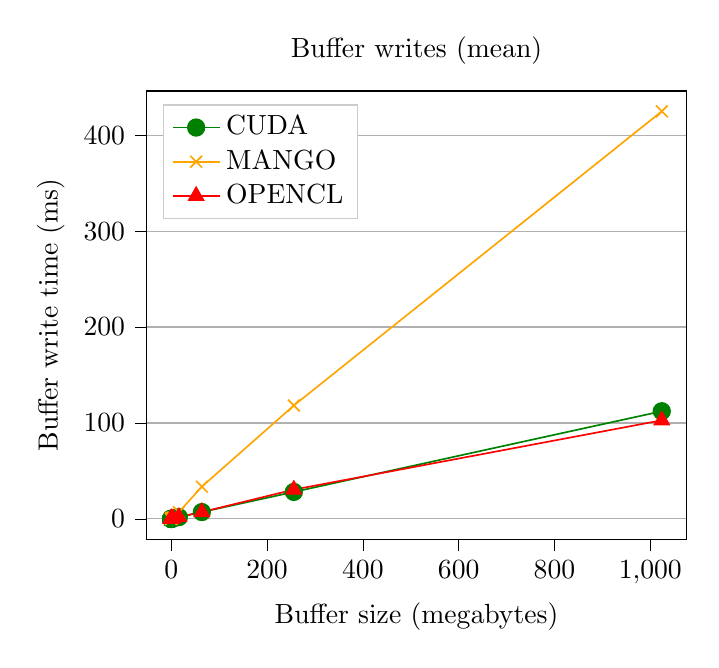
\begin{tikzpicture}

\definecolor{color0}{rgb}{1,0.647058823529412,0}

\begin{axis}[
legend cell align={left},
legend style={
  fill opacity=1,
  draw opacity=1,
  text opacity=1,
  at={(0.03,0.97)},
  anchor=north west,
  draw=white!80!black
},
tick align=outside,
tick pos=left,
title={Buffer writes (mean)},
x grid style={white!69.0196078431373!black},
xlabel={Buffer size (megabytes)},
xmin=-51.195849609375, xmax=1075.13432617188,
xtick style={color=black},
y grid style={white!69.0196078431373!black},
ylabel={Buffer write time (ms)},
ymajorgrids,
ymin=-21.2301063907143, ymax=446.080604551939,
ytick style={color=black},
yticklabel style={/pgf/number format/fixed},
]
\addplot [semithick, green!50.1960784313725!black, mark=*, mark size=3, mark options={solid}]
table {%
0.0009765625 0.0112895612244898
0.001953125 0.01208368
0.00390625 0.0117242333333333
0.0078125 0.0129084736842105
0.015625 0.01453375
0.03125 0.0176991
0.0625 0.0208775
0.2490234375 0.0286712755102041
0.998046875 0.10126693877551
3.99609375 0.459110655172414
15.9921875 1.80984045
63.984375 7.13521621052632
255.96875 28.1117542
1023.9375 112.2217462
};
\addlegendentry{CUDA}
\addplot [semithick, color0, mark=x, mark size=3, mark options={solid}]
table {%
0.0009765625 0.17391198989899
0.001953125 0.17851804
0.00390625 0.165922633333333
0.0078125 0.1528704
0.015625 0.1705615
0.03125 0.1738537
0.0625 0.7945439
0.2490234375 0.300501707070707
0.998046875 0.60951162
3.99609375 1.45868382758621
15.9921875 7.00193921052632
63.984375 33.6318241
255.96875 118.210402
1023.9375 424.8392086
};
\addlegendentry{MANGO}
\addplot [semithick, red, mark=triangle*, mark size=3, mark options={solid}]
table {%
0.0009765625 0.21893114
0.001953125 0.21817348
0.00390625 0.226192172413793
0.0078125 0.22287355
0.015625 0.2213049
0.03125 0.2202647
0.0625 0.2337682
0.2490234375 0.0643956597938144
0.998046875 0.19593170212766
3.99609375 0.621945551724138
15.9921875 1.96354655
63.984375 7.15548315
255.96875 30.5490241
1023.9375 102.7730812
};
\addlegendentry{OPENCL}
\end{axis}

\end{tikzpicture}

    } 
    }}%
    \qquad
    \subfloat[\centering Mean buffer read time]{{
        \resizebox{!}{160pt}{
            % This file was created by tikzplotlib v0.9.8.
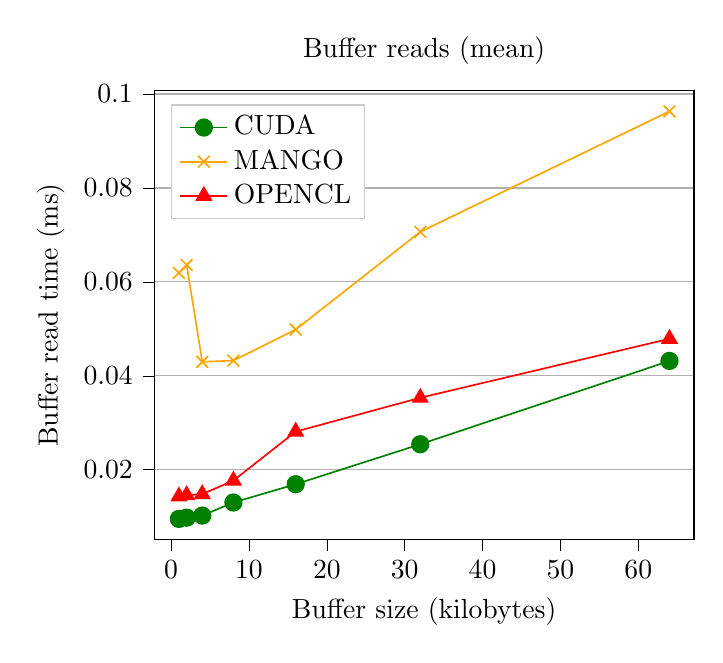
\begin{tikzpicture}

\definecolor{color0}{rgb}{1,0.647058823529412,0}

\begin{axis}[
legend cell align={left},
legend style={
  fill opacity=1,
  draw opacity=1,
  text opacity=1,
  at={(0.03,0.97)},
  anchor=north west,
  draw=white!80!black
},
tick align=outside,
tick pos=left,
title={Buffer reads (mean)},
x grid style={white!69.0196078431373!black},
xlabel={Buffer size (kilobytes)},
xmin=-2.15, xmax=67.15,
xtick style={color=black},
y grid style={white!69.0196078431373!black},
ylabel={Buffer read time (ms)},
ymajorgrids,
ymin=0.00520630214285714, ymax=0.100653614183673,
ytick style={color=black},
yticklabel style={/pgf/number format/fixed},
]
\addplot [semithick, green!50.1960784313725!black, mark=*, mark size=3, mark options={solid}]
table {%
1 0.00954481632653061
2 0.0097984693877551
4 0.0102500714285714
8 0.01303545
16 0.01692725
32 0.0254355
64 0.0431711
};
\addlegendentry{CUDA}
\addplot [semithick, color0, mark=x, mark size=3, mark options={solid}]
table {%
1 0.0619118
2 0.06359902
4 0.0429807333333333
8 0.0432455789473684
16 0.04984925
32 0.0706595
64 0.0963151
};
\addlegendentry{MANGO}
\addplot [semithick, red, mark=triangle*, mark size=3, mark options={solid}]
table {%
1 0.0143187777777778
2 0.01460112
4 0.0148169
8 0.01770105
16 0.02812495
32 0.0353335
64 0.0478901
};
\addlegendentry{OPENCL}
\end{axis}

\end{tikzpicture}

        } 
    }}%
    \captionsetup{justification=centering}
    \caption{Mean buffer transfer times for PathFinder}%
    \label{fig:pathfinder_buffer_transfers_mean}%
\end{figure}

Finally, we move on to the benchmark breakdown which, similarly to the one for HotSpot, is generated with the largest input size for PathFinder, 16384 x 16384. Here in figure \ref{fig:pathfinder_breakdown} we can clearly see that the factor that most contributes to the difference in performance between the different implementations are actually the miscellaneous tasks (plus resource allocation for MANGO), taking up around 50\% of the running time. These include all the boilerplate and preparations required to setup the different execution environments. While this is very minimal in the case of CUDA, as it is a single-source model, where kernel and host code are precompiled and loaded together, the setup is much more significant for MANGO and OpenCL. Both OpenCL and MANGO require loading a separate kernel file, requiring I/O operations. After that OpenCL also adds kernel compilation and device setup, while MANGO requires communication with BBQUE to perform resource allocation and deallocation. These aspects are not significant for HotSpot as the total running time is much longer and the overhead of the setup is constant, no matter the input size.

\begin{figure}
    \centering
    \resizebox{!}{160pt}{
        % This file was created by tikzplotlib v0.9.8.
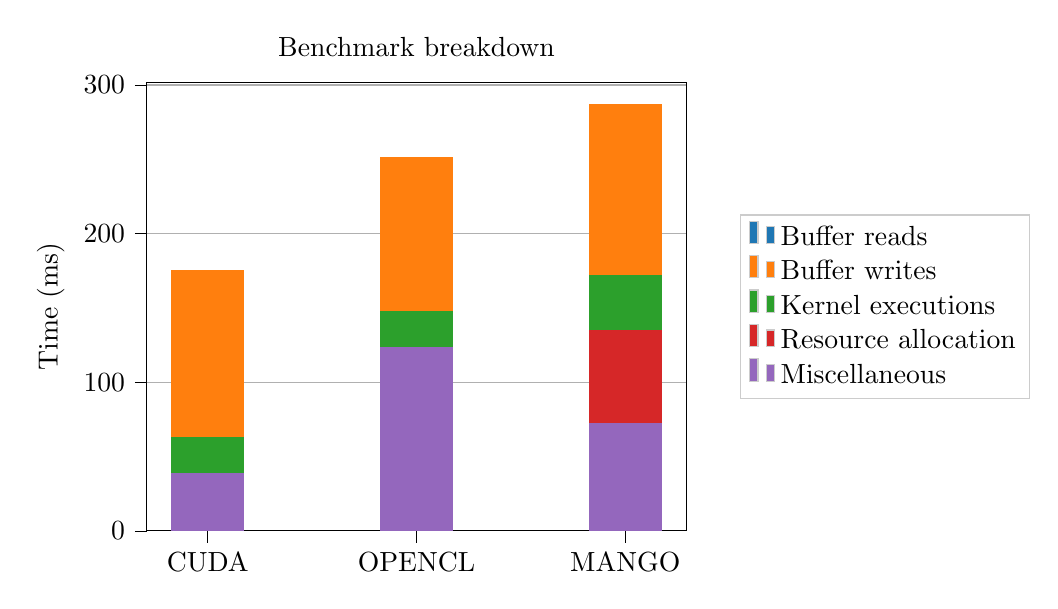
\begin{tikzpicture}

\definecolor{color0}{rgb}{0.12156862745098,0.466666666666667,0.705882352941177}
\definecolor{color1}{rgb}{1,0.498039215686275,0.0549019607843137}
\definecolor{color2}{rgb}{0.172549019607843,0.627450980392157,0.172549019607843}
\definecolor{color3}{rgb}{0.83921568627451,0.152941176470588,0.156862745098039}
\definecolor{color4}{rgb}{0.580392156862745,0.403921568627451,0.741176470588235}

\begin{axis}[
legend cell align={left},
legend style={
  fill opacity=1,
  draw opacity=1,
  text opacity=1,
  at={(1.1,0.5)},
  anchor=west,
  draw=white!80!black
},
tick align=outside,
tick pos=left,
title={Benchmark breakdown},
x grid style={white!69.0196078431373!black},
xmin=-0.2925, xmax=2.2925,
xtick style={color=black},
xtick={0,1,2},
xticklabels={CUDA,OPENCL,MANGO},
y grid style={white!69.0196078431373!black},
ylabel={Time (ms)},
ymajorgrids,
ymin=0, ymax=301.689864945,
ytick style={color=black}
]
\draw[draw=none,fill=color0] (axis cs:-0.175,175.3350163) rectangle (axis cs:0.175,175.3781874);
\addlegendimage{ybar,ybar legend,draw=none,fill=color0};
\addlegendentry{Buffer reads}

\draw[draw=none,fill=color0] (axis cs:0.825,251.2425685) rectangle (axis cs:1.175,251.2904586);
\draw[draw=none,fill=color0] (axis cs:1.825,287.2901947) rectangle (axis cs:2.175,287.3236809);
\draw[draw=none,fill=color1] (axis cs:-0.175,63.0923926) rectangle (axis cs:0.175,175.3350163);
\addlegendimage{ybar,ybar legend,draw=none,fill=color1};
\addlegendentry{Buffer writes}

\draw[draw=none,fill=color1] (axis cs:0.825,148.2357191) rectangle (axis cs:1.175,251.2425685);
\draw[draw=none,fill=color1] (axis cs:1.825,172.0310368) rectangle (axis cs:2.175,287.2901947);
\draw[draw=none,fill=color2] (axis cs:-0.175,38.8204022) rectangle (axis cs:0.175,63.0923926);
\addlegendimage{ybar,ybar legend,draw=none,fill=color2};
\addlegendentry{Kernel executions}

\draw[draw=none,fill=color2] (axis cs:0.825,123.4029374) rectangle (axis cs:1.175,148.2357191);
\draw[draw=none,fill=color2] (axis cs:1.825,134.9503335) rectangle (axis cs:2.175,172.0310368);
\draw[draw=none,fill=color3] (axis cs:-0.175,38.8204022) rectangle (axis cs:0.175,38.8204022);
\addlegendimage{ybar,ybar legend,draw=none,fill=color3};
\addlegendentry{Resource allocation}

\draw[draw=none,fill=color3] (axis cs:0.825,123.4029374) rectangle (axis cs:1.175,123.4029374);
\draw[draw=none,fill=color3] (axis cs:1.825,72.350049) rectangle (axis cs:2.175,134.9503335);
\draw[draw=none,fill=color4] (axis cs:-0.175,0) rectangle (axis cs:0.175,38.8204022);
\addlegendimage{ybar,ybar legend,draw=none,fill=color4};
\addlegendentry{Miscellaneous}

\draw[draw=none,fill=color4] (axis cs:0.825,0) rectangle (axis cs:1.175,123.4029374);
\draw[draw=none,fill=color4] (axis cs:1.825,0) rectangle (axis cs:2.175,72.350049);
\end{axis}

\end{tikzpicture}

    }
    \captionsetup{justification=centering}
    \caption{Benchmark breakdown for PathFinder}
    \label{fig:pathfinder_breakdown}
\end{figure}

\subsubsection{AXPY}

In AXPY we move straight to the mean kernel execution time in figure \ref{fig:axpy_kernel_executions_mean} where we can see that CUDA performs 12.4\% faster than MANGO, while OpenCL is only 7\% faster for the same size input.

\begin{figure}
    \centering
    \resizebox{!}{160pt}{
        % This file was created by tikzplotlib v0.9.8.
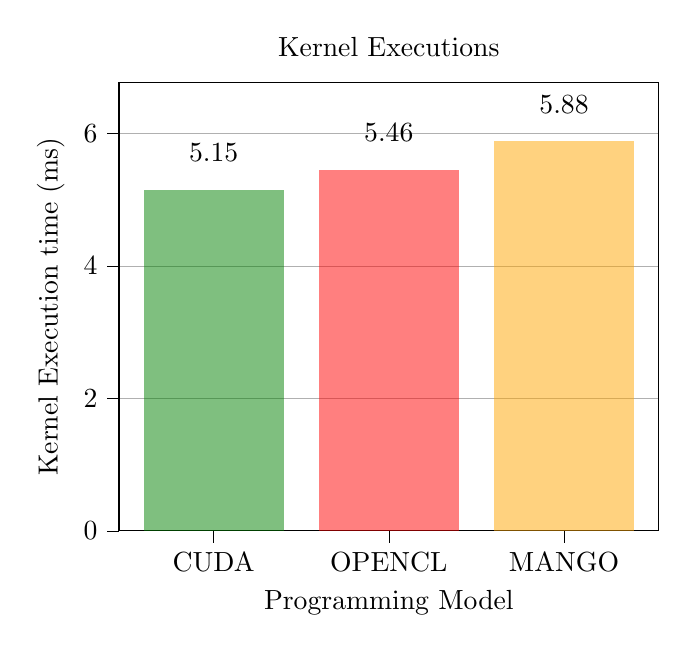
\begin{tikzpicture}

\definecolor{color0}{rgb}{1,0.647058823529412,0}

\begin{axis}[
tick align=outside,
tick pos=left,
title={Kernel Executions},
x grid style={white!69.0196078431373!black},
xlabel={Programming Model},
xmin=-0.54, xmax=2.54,
xtick style={color=black},
xtick={0,1,2},
xticklabels={CUDA,OPENCL,MANGO},
y grid style={white!69.0196078431373!black},
ylabel={Kernel Execution time (ms)},
ymajorgrids,
ymin=0, ymax=6.7738881661,
ytick style={color=black}
]
\draw[draw=none,fill=green!50.1960784313725!black,fill opacity=0.5] (axis cs:-0.4,0) rectangle (axis cs:0.4,5.15266011);
\draw[draw=none,fill=red,fill opacity=0.5] (axis cs:0.6,0) rectangle (axis cs:1.4,5.45583448);
\draw[draw=none,fill=color0,fill opacity=0.5] (axis cs:1.6,0) rectangle (axis cs:2.4,5.88321827);
\draw (axis cs:0,5.427521991) node[
  scale=1,
  anchor=south,
  text=black,
  rotate=0.0
]{5.15};
\draw (axis cs:1,5.730696361) node[
  scale=1,
  anchor=south,
  text=black,
  rotate=0.0
]{5.46};
\draw (axis cs:2,6.158080151) node[
  scale=1,
  anchor=south,
  text=black,
  rotate=0.0
]{5.88};
\end{axis}

\end{tikzpicture}

    }
    \captionsetup{justification=centering}
    \caption{Mean kernel execution times for AXPY}
    \label{fig:axpy_kernel_executions_mean}
\end{figure}

As we know that AXPY is purely memory bandwidth bound, we can translate this kernel execution times to memory bandwidth measurements as seen in figure \ref{fig:axpy_bandwidth_mean}. In this figure we can see the percentage of theoretical peak bandwidth achieved by each programming model.

\begin{figure}
    \centering
    \resizebox{!}{160pt}{
        % This file was created by tikzplotlib v0.9.8.
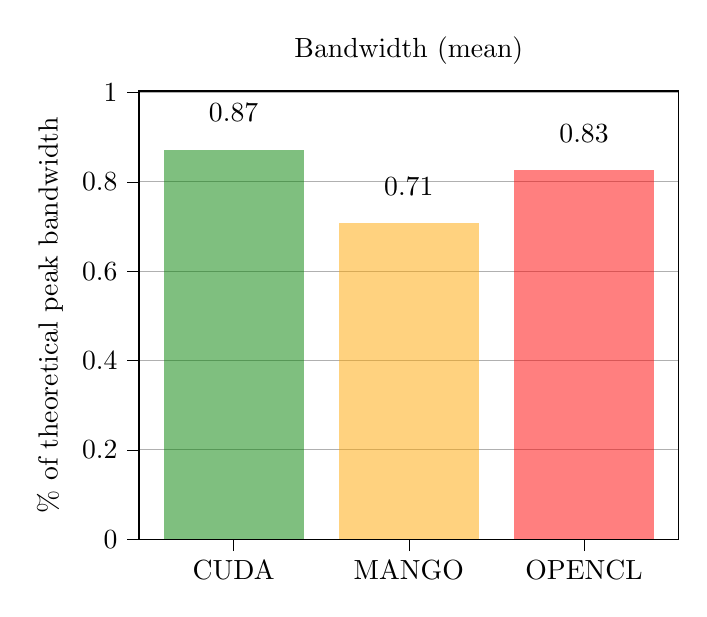
\begin{tikzpicture}

\definecolor{color0}{rgb}{1,0.647058823529412,0}

\begin{axis}[
tick align=outside,
tick pos=left,
title={Bandwidth (mean)},
x grid style={white!69.0196078431373!black},
xmin=-0.54, xmax=2.54,
xtick style={color=black},
xtick={0,1,2},
xticklabels={CUDA,MANGO,OPENCL},
y grid style={white!69.0196078431373!black},
ylabel={\% of theoretical peak bandwidth},
ymajorgrids,
ymin=0, ymax=1.00347644198507,
ytick style={color=black},
yticklabel style={/pgf/number format/fixed},
]
\draw[draw=none,fill=green!50.1960784313725!black,fill opacity=0.5] (axis cs:-0.4,0) rectangle (axis cs:0.4,0.872156563953115);
\draw[draw=none,fill=color0,fill opacity=0.5] (axis cs:0.6,0) rectangle (axis cs:1.4,0.707407075302276);
\draw[draw=none,fill=red,fill opacity=0.5] (axis cs:1.6,0) rectangle (axis cs:2.4,0.826121177288947);
\draw (axis cs:0,0.91225131089552) node[
  scale=1,
  anchor=south,
  text=black,
  rotate=0.0
]{0.87};
\draw (axis cs:1,0.747501822244682) node[
  scale=1,
  anchor=south,
  text=black,
  rotate=0.0
]{0.71};
\draw (axis cs:2,0.866215924231353) node[
  scale=1,
  anchor=south,
  text=black,
  rotate=0.0
]{0.83};
\end{axis}

\end{tikzpicture}

    }
    \captionsetup{justification=centering}
    \caption{Mean GPU memory bandwidth for AXPY}
    \label{fig:axpy_bandwidth_mean}
\end{figure}

What is interesting is that if we look at the maximum bandwidth achieved by each model MANGO is able to beat both CUDA and OpenCL, being 1\% and 4.5\% faster than each programming model respectively. This indicates that our implementation does not inherently pose a limit to the performance that could be achieved by the GPU when compared to pure CUDA and the overhead is likely affected by varying external factors, such as background processes or Operating System context switches. 

\begin{figure}
    \centering
    \resizebox{!}{160pt}{
        % This file was created by tikzplotlib v0.9.8.
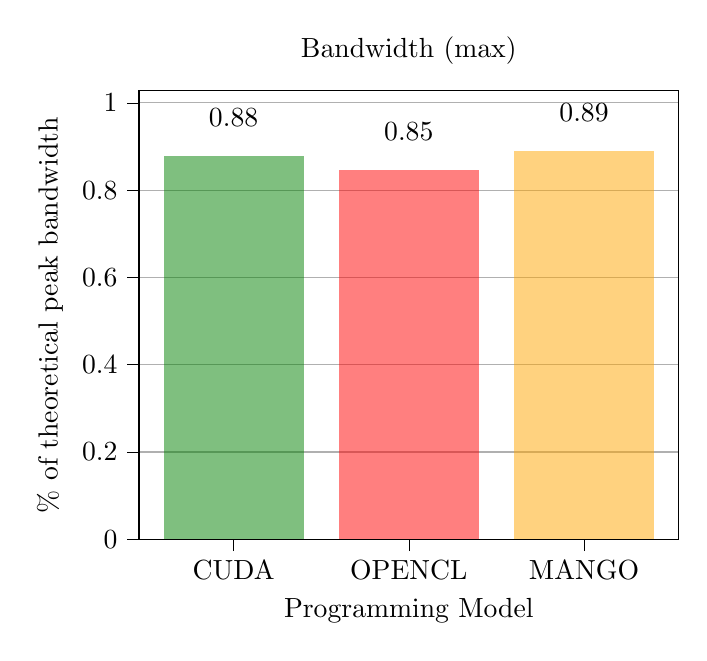
\begin{tikzpicture}

\definecolor{color0}{rgb}{1,0.647058823529412,0}

\begin{axis}[
tick align=outside,
tick pos=left,
title={Bandwidth (max)},
x grid style={white!69.0196078431373!black},
xlabel={Programming Model},
xmin=-0.54, xmax=2.54,
xtick style={color=black},
xtick={0,1,2},
xticklabels={CUDA,OPENCL,MANGO},
y grid style={white!69.0196078431373!black},
ylabel={\% of theoretical peak bandwidth},
ymajorgrids,
ymin=0, ymax=1.02734953480631,
ytick style={color=black}
]
\draw[draw=none,fill=green!50.1960784313725!black,fill opacity=0.5] (axis cs:-0.4,0) rectangle (axis cs:0.4,0.87937553130392);
\draw[draw=none,fill=red,fill opacity=0.5] (axis cs:0.6,0) rectangle (axis cs:1.4,0.846996642648818);
\draw[draw=none,fill=color0,fill opacity=0.5] (axis cs:1.6,0) rectangle (axis cs:2.4,0.890342216051125);
\draw (axis cs:0,0.922987437803984) node[
  scale=1,
  anchor=south,
  text=black,
  rotate=0.0
]{0.88};
\draw (axis cs:1,0.890608549148883) node[
  scale=1,
  anchor=south,
  text=black,
  rotate=0.0
]{0.85};
\draw (axis cs:2,0.933954122551189) node[
  scale=1,
  anchor=south,
  text=black,
  rotate=0.0
]{0.89};
\end{axis}

\end{tikzpicture}

    }
    \captionsetup{justification=centering}
    \caption{Max GPU memory bandwidth for AXPY}
    \label{fig:axpy_bandwidth_max}
\end{figure}

Finally, we look at the transfer times achieved between the host and the device and vice versa and how these translate to the percentage of PCI-E bandwidth achieved. These comparisons can be seen in figures \ref{fig:axpy_buffer_transfers_mean} and \ref{fig:axpy_buffer_transfers_bandwidth_mean} respectively. In terms of device-to-host transfers, the difference in performance is negligible, although none of the models provide an optimal speed for the available PCI-E connection. For host-to-device transfers, MANGO gets second place, with CUDA being 6\% faster and OpenCL 7\% slower. Still, none of the models achieve close to maximum usage of the PCI-E connection.

\begin{figure}%
    \centering
    \subfloat[\centering Mean buffer write time]{{
        \resizebox{!}{160pt}{
        % This file was created by tikzplotlib v0.9.8.
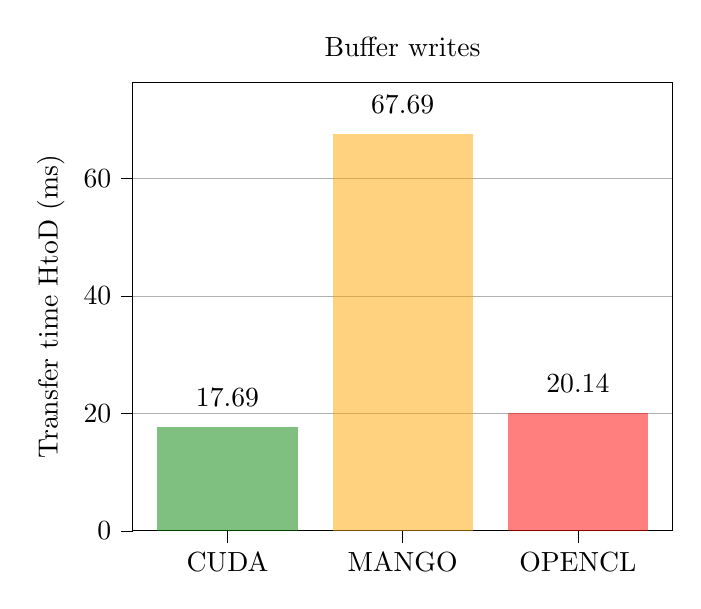
\begin{tikzpicture}

\definecolor{color0}{rgb}{1,0.647058823529412,0}

\begin{axis}[
tick align=outside,
tick pos=left,
title={Buffer writes},
x grid style={white!69.0196078431373!black},
xmin=-0.54, xmax=2.54,
xtick style={color=black},
xtick={0,1,2},
xticklabels={CUDA,MANGO,OPENCL},
y grid style={white!69.0196078431373!black},
ylabel={Transfer time HtoD (ms)},
ymajorgrids,
ymin=0, ymax=76.3910404992625,
ytick style={color=black},
yticklabel style={/pgf/number format/fixed},
]
\draw[draw=none,fill=green!50.1960784313725!black,fill opacity=0.5] (axis cs:-0.4,0) rectangle (axis cs:0.4,17.68977225);
\draw[draw=none,fill=color0,fill opacity=0.5] (axis cs:0.6,0) rectangle (axis cs:1.4,67.6877919275);
\draw[draw=none,fill=red,fill opacity=0.5] (axis cs:1.6,0) rectangle (axis cs:2.4,20.138947405);
\draw (axis cs:0,19.448380776375) node[
  scale=1,
  anchor=south,
  text=black,
  rotate=0.0
]{17.69};
\draw (axis cs:1,69.446400453875) node[
  scale=1,
  anchor=south,
  text=black,
  rotate=0.0
]{67.69};
\draw (axis cs:2,21.897555931375) node[
  scale=1,
  anchor=south,
  text=black,
  rotate=0.0
]{20.14};
\end{axis}

\end{tikzpicture}

    } 
    }}%
    \qquad
    \subfloat[\centering Mean buffer read time]{{
        \resizebox{!}{160pt}{
            % This file was created by tikzplotlib v0.9.8.
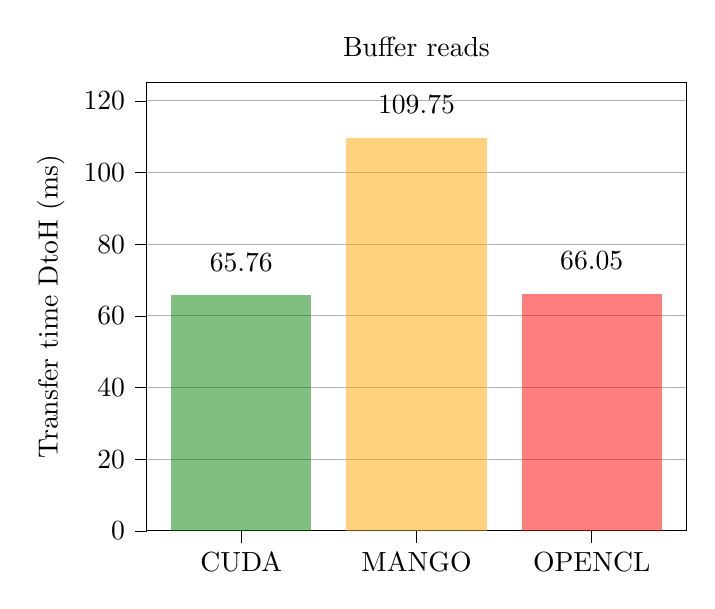
\begin{tikzpicture}

\definecolor{color0}{rgb}{1,0.647058823529412,0}

\begin{axis}[
tick align=outside,
tick pos=left,
title={Buffer reads},
x grid style={white!69.0196078431373!black},
xmin=-0.54, xmax=2.54,
xtick style={color=black},
xtick={0,1,2},
xticklabels={CUDA,MANGO,OPENCL},
y grid style={white!69.0196078431373!black},
ylabel={Transfer time DtoH (ms)},
ymajorgrids,
ymin=0, ymax=125.150330663325,
ytick style={color=black},
yticklabel style={/pgf/number format/fixed},
]
\draw[draw=none,fill=green!50.1960784313725!black,fill opacity=0.5] (axis cs:-0.4,0) rectangle (axis cs:0.4,65.76414157);
\draw[draw=none,fill=color0,fill opacity=0.5] (axis cs:0.6,0) rectangle (axis cs:1.4,109.746946745);
\draw[draw=none,fill=red,fill opacity=0.5] (axis cs:1.6,0) rectangle (axis cs:2.4,66.05377953);
\draw (axis cs:0,69.79022270075) node[
  scale=1,
  anchor=south,
  text=black,
  rotate=0.0
]{65.76};
\draw (axis cs:1,113.77302787575) node[
  scale=1,
  anchor=south,
  text=black,
  rotate=0.0
]{109.75};
\draw (axis cs:2,70.07986066075) node[
  scale=1,
  anchor=south,
  text=black,
  rotate=0.0
]{66.05};
\end{axis}

\end{tikzpicture}

        } 
    }}%
    \captionsetup{justification=centering}
    \caption{Mean buffer transfer times for AXPY}%
    \label{fig:axpy_buffer_transfers_mean}%
\end{figure}

\begin{figure}%
    \centering
    \subfloat[\centering Mean host to device transfer bandwidth]{{
        \resizebox{!}{160pt}{
        % This file was created by tikzplotlib v0.9.8.
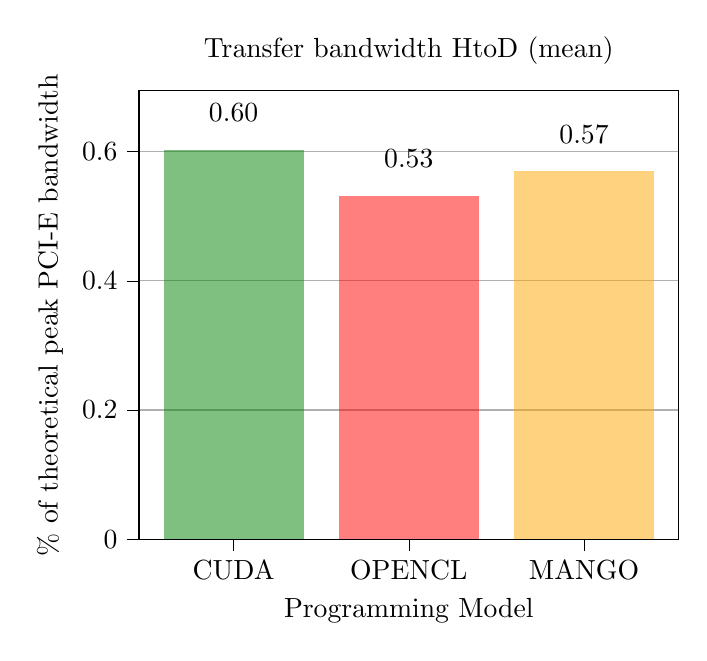
\begin{tikzpicture}

\definecolor{color0}{rgb}{1,0.647058823529412,0}

\begin{axis}[
tick align=outside,
tick pos=left,
title={Transfer bandwidth HtoD (mean)},
x grid style={white!69.0196078431373!black},
xlabel={Programming Model},
xmin=-0.54, xmax=2.54,
xtick style={color=black},
xtick={0,1,2},
xticklabels={CUDA,OPENCL,MANGO},
y grid style={white!69.0196078431373!black},
ylabel={\% of theoretical peak PCI-E bandwidth},
ymajorgrids,
ymin=0, ymax=0.693817866752193,
ytick style={color=black}
]
\draw[draw=none,fill=green!50.1960784313725!black,fill opacity=0.5] (axis cs:-0.4,0) rectangle (axis cs:0.4,0.602361171863845);
\draw[draw=none,fill=red,fill opacity=0.5] (axis cs:0.6,0) rectangle (axis cs:1.4,0.53135754934798);
\draw[draw=none,fill=color0,fill opacity=0.5] (axis cs:1.6,0) rectangle (axis cs:2.4,0.569221880713467);
\draw (axis cs:0,0.630743515229267) node[
  scale=1,
  anchor=south,
  text=black,
  rotate=0.0
]{0.60};
\draw (axis cs:1,0.559739892713401) node[
  scale=1,
  anchor=south,
  text=black,
  rotate=0.0
]{0.53};
\draw (axis cs:2,0.597604224078889) node[
  scale=1,
  anchor=south,
  text=black,
  rotate=0.0
]{0.57};
\end{axis}

\end{tikzpicture}

    } 
    }}%
    \qquad
    \subfloat[\centering Mean device to host transfer bandwidth]{{
        \resizebox{!}{160pt}{
            % This file was created by tikzplotlib v0.9.8.
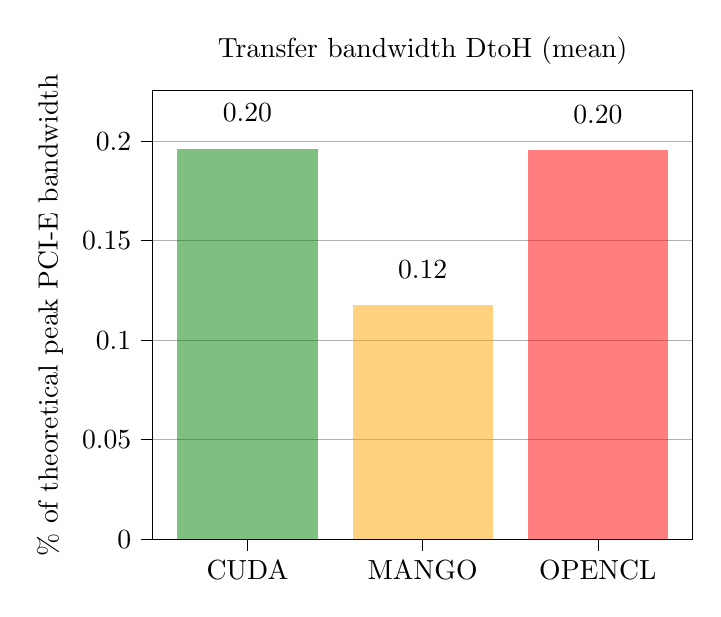
\begin{tikzpicture}

\definecolor{color0}{rgb}{1,0.647058823529412,0}

\begin{axis}[
tick align=outside,
tick pos=left,
title={Transfer bandwidth DtoH (mean)},
x grid style={white!69.0196078431373!black},
xmin=-0.54, xmax=2.54,
xtick style={color=black},
xtick={0,1,2},
xticklabels={CUDA,MANGO,OPENCL},
y grid style={white!69.0196078431373!black},
ylabel={\% of theoretical peak PCI-E bandwidth},
ymajorgrids,
ymin=0, ymax=0.225207888741475,
ytick style={color=black},
yticklabel style={/pgf/number format/fixed},
]
\draw[draw=none,fill=green!50.1960784313725!black,fill opacity=0.5] (axis cs:-0.4,0) rectangle (axis cs:0.4,0.196246840753961);
\draw[draw=none,fill=color0,fill opacity=0.5] (axis cs:0.6,0) rectangle (axis cs:1.4,0.11760810305661);
\draw[draw=none,fill=red,fill opacity=0.5] (axis cs:1.6,0) rectangle (axis cs:2.4,0.195401269577688);
\draw (axis cs:0,0.204734444310432) node[
  scale=1,
  anchor=south,
  text=black,
  rotate=0.0
]{0.20};
\draw (axis cs:1,0.126095706613081) node[
  scale=1,
  anchor=south,
  text=black,
  rotate=0.0
]{0.12};
\draw (axis cs:2,0.203888873134159) node[
  scale=1,
  anchor=south,
  text=black,
  rotate=0.0
]{0.20};
\end{axis}

\end{tikzpicture}

        } 
    }}%
    \captionsetup{justification=centering}
    \caption{Mean buffer transfer bandwidths for AXPY}%
    \label{fig:axpy_buffer_transfers_bandwidth_mean}%
\end{figure}

\subsection{IPC}

As mentioned in section \ref{sect:setup-methodology}, the previous benchmarks did not take into account the overhead added by inter process communication between the libmango client and the HHAL server. Here we will focus on this part separately to evaluate our communication scheme and how it can be improved.

Starting with figure \ref{fig:hotspot_total_and_kernel_executions_mean_ipc} we can see how the total duration of the HotSpot benchmark increases when taking IPC into account, and how this difference scales with larger input sizes. This however is not linked with the kernel execution time, which is perfectly in line with the benchmark without any IPC. 

\begin{figure}%
    \centering
    \subfloat[\centering Mean total execution time]{{
        \resizebox{!}{160pt}{
        % This file was created by tikzplotlib v0.9.8.
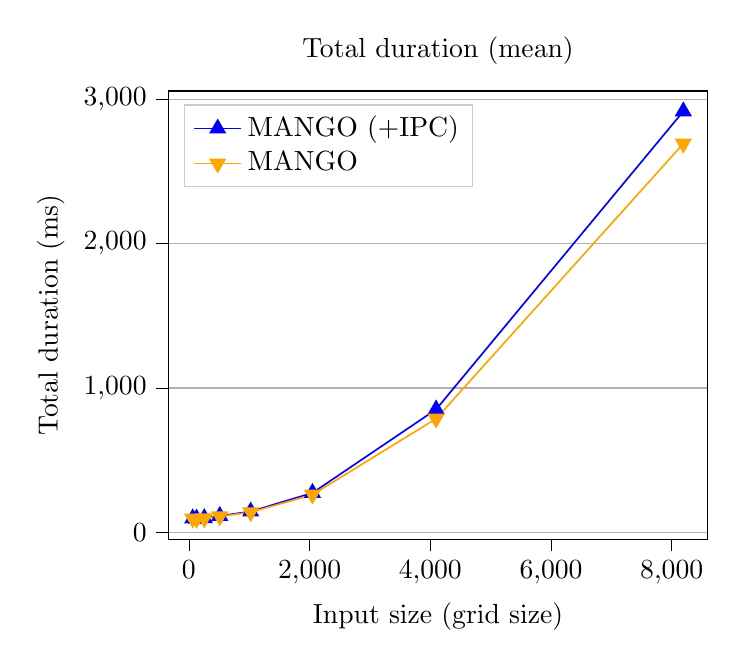
\begin{tikzpicture}

\definecolor{color0}{rgb}{1,0.647058823529412,0}

\begin{axis}[
legend cell align={left},
legend style={
  fill opacity=1,
  draw opacity=1,
  text opacity=1,
  at={(0.03,0.97)},
  anchor=north west,
  draw=white!80!black
},
tick align=outside,
tick pos=left,
title={Total duration (mean)},
x grid style={white!69.0196078431373!black},
xlabel={Input size (grid size)},
xmin=-342.4, xmax=8598.4,
xtick style={color=black},
y grid style={white!69.0196078431373!black},
ylabel={Total duration (ms)},
ymajorgrids,
ymin=-47.709970137, ymax=3056.950953997,
ytick style={color=black}
]
\addplot [semithick, blue, mark=triangle*, mark size=3, mark options={solid}]
table {%
64 97.31526544
128 95.37001074
256 98.8516923
512 114.4259599
1024 144.57944185
2048 273.3834686
4096 851.6563961
8192 2915.8300029
};
\addlegendentry{MANGO (+IPC)}
\addplot [semithick, color0, mark=triangle*, mark size=3, mark options={solid,rotate=180}]
table {%
64 95.13603588
128 93.41098096
256 96.4721031
512 110.236007833333
1024 139.4998439
2048 261.1760106
4096 787.2880039
8192 2692.1909758
};
\addlegendentry{MANGO}
\end{axis}

\end{tikzpicture}

    } 
    }}%
    \qquad
    \subfloat[\centering Mean kernel execution time]{{
        \resizebox{!}{160pt}{
            % This file was created by tikzplotlib v0.9.8.
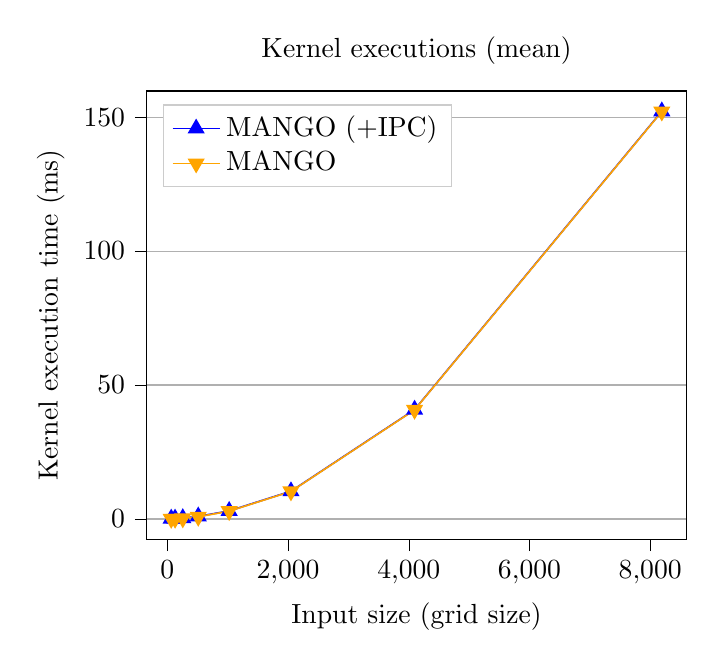
\begin{tikzpicture}

\definecolor{color0}{rgb}{1,0.647058823529412,0}

\begin{axis}[
legend cell align={left},
legend style={
  fill opacity=1,
  draw opacity=1,
  text opacity=1,
  at={(0.03,0.97)},
  anchor=north west,
  draw=white!80!black
},
tick align=outside,
tick pos=left,
title={Kernel executions (mean)},
x grid style={white!69.0196078431373!black},
xlabel={Input size (grid size)},
xmin=-342.4, xmax=8598.4,
xtick style={color=black},
y grid style={white!69.0196078431373!black},
ylabel={Kernel execution time (ms)},
ymajorgrids,
ymin=-7.56409453556224, ymax=159.757092421107,
ytick style={color=black}
]
\addplot [semithick, blue, mark=triangle*, mark size=3, mark options={solid}]
table {%
64 0.160601098734177
128 0.169648774647887
256 0.323446888888889
512 0.96640755075594
1024 3.01892553968254
2048 10.357626175
4096 40.811188164557
8192 152.151583923077
};
\addlegendentry{MANGO (+IPC)}
\addplot [semithick, color0, mark=triangle*, mark size=3, mark options={solid,rotate=180}]
table {%
64 0.0414139624681934
128 0.0703628888888889
256 0.211658812903226
512 0.81808229004329
1024 2.9290935968254
2048 10.27900955
4096 40.7308336708861
8192 152.061428076923
};
\addlegendentry{MANGO}
\end{axis}

\end{tikzpicture}

        } 
    }}%
    \captionsetup{justification=centering}
    \caption{Mean total and kernel execution times for HotSpot}%
    \label{fig:hotspot_total_and_kernel_executions_mean_ipc}%
\end{figure}

For the same metrics, PathFinder sees a much steeper increase in total running time along with the execution time. As can be see in figure \ref{fig:pathfinder_total_and_kernel_executions_mean_ipc}b, this is more closely linked with the kernel execution time which here shows a clear separation between IPC and no IPC. In addition, the PathFinder kernel is run more times as the input size increases, so this overhead piles up with multiple executions.

If we compare these results with the ones in HotSpot, we can conclude that the overhead experienced with IPC is fixed and does not scale with input size. This is supported by the fact that HotSpot kernel executions are an order of magnitude larger than PathFinder executions (150ms for HotSpot versus 90/40 $\mu$s for PathFinder).

\begin{figure}%
    \centering
    \subfloat[\centering Mean total execution time]{{
        \resizebox{!}{160pt}{
        % This file was created by tikzplotlib v0.9.8.
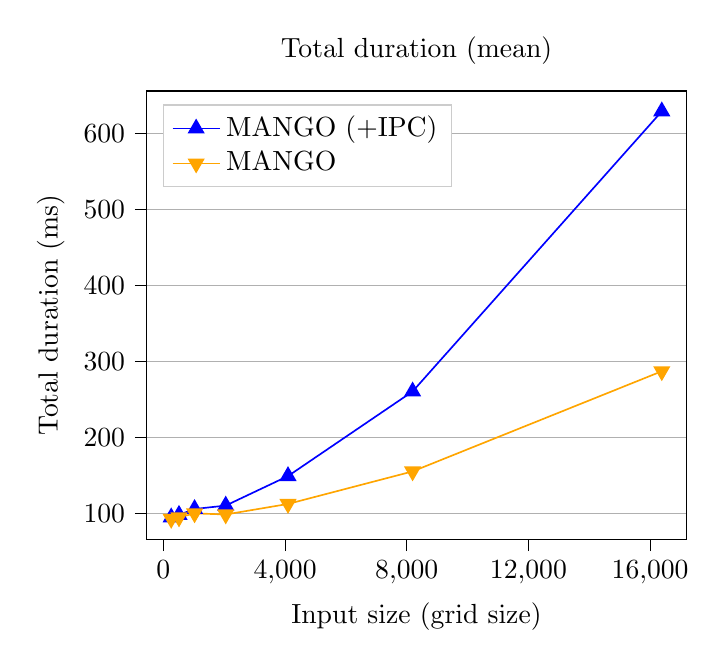
\begin{tikzpicture}

\definecolor{color0}{rgb}{1,0.647058823529412,0}

\begin{axis}[
legend cell align={left},
legend style={
  fill opacity=1,
  draw opacity=1,
  text opacity=1,
  at={(0.03,0.97)},
  anchor=north west,
  draw=white!80!black
},
tick align=outside,
tick pos=left,
title={Total duration (mean)},
x grid style={white!69.0196078431373!black},
xlabel={Input size (grid size)},
xmin=-550.4, xmax=17190.4,
xtick style={color=black},
y grid style={white!69.0196078431373!black},
ylabel={Total duration (ms)},
ymajorgrids,
ymin=66.2281451992424, ymax=656.161493704798,
ytick style={color=black},
scaled x ticks = false,
xtick={0, 4000, 8000, 12000, 16000},
]
\addplot [semithick, blue, mark=triangle*, mark size=3, mark options={solid}]
table {%
256 95.08814335
512 98.3987611428572
1024 106.0719735
2048 110.582484578947
4096 149.39266355
8192 260.7485585
16384 629.3463415
};
\addlegendentry{MANGO (+IPC)}
\addplot [semithick, color0, mark=triangle*, mark size=3, mark options={solid,rotate=180}]
table {%
256 93.0432974040404
512 94.9890068367347
1024 100.334116733333
2048 98.8606154736842
4096 112.71933675
8192 155.5354245
16384 287.3236809
};
\addlegendentry{MANGO}
\end{axis}

\end{tikzpicture}

    } 
    }}%
    \qquad
    \subfloat[\centering Mean kernel execution time]{{
        \resizebox{!}{160pt}{
            % This file was created by tikzplotlib v0.9.8.
\begin{tikzpicture}

\definecolor{color0}{rgb}{1,0.647058823529412,0}

\begin{axis}[
legend cell align={left},
legend style={fill opacity=1, draw opacity=1, text opacity=1, draw=white!80!black},
tick align=outside,
tick pos=left,
title={Kernel executions (mean)},
x grid style={white!69.0196078431373!black},
xlabel={Input size (grid size)},
xmin=-550.4, xmax=17190.4,
xtick style={color=black},
y grid style={white!69.0196078431373!black},
ylabel={Kernel execution time (μs)},
ymajorgrids,
ymin=20.0751821021274, ymax=154.280935499242,
ytick style={color=black},
scaled x ticks = false,
xtick={0, 4000, 8000, 12000, 16000},
]
\addplot [semithick, blue, mark=triangle*, mark size=3, mark options={solid}]
table {%
256 148.180673981191
512 147.824040880503
1024 115.638007251154
2048 84.3323422222222
4096 88.6508752789487
8192 85.3244863861386
16384 90.6984343047666
};
\addlegendentry{MANGO (+IPC)}
\addplot [semithick, color0, mark=triangle*, mark size=3, mark options={solid,rotate=180}]
table {%
256 35.8026210691824
512 35.0376165354331
1024 32.4320626649077
2048 26.175443620178
4096 27.2096125186289
8192 28.3202890760466
16384 36.8636978381717
};
\addlegendentry{MANGO}
\end{axis}

\end{tikzpicture}

        } 
    }}%
    \captionsetup{justification=centering}
    \caption{Mean total and kernel execution times for PathFinder}%
    \label{fig:pathfinder_total_and_kernel_executions_mean_ipc}%
\end{figure}

Buffer transfers, as expected, are affected significantly more by IPC as the amount of data that needs to be transferred is much higher than what is needed to launch a kernel. Both figure \ref{fig:hotspot_buffer_transfers_mean_ipc} and figure \ref{fig:pathfinder_buffer_transfers_mean_ipc} show similar scaling for buffer writes. There is a clear discrepancy between the buffer reads, however this can be attributed to the considerable difference in buffer sizes.


\begin{figure}%
    \centering
    \subfloat[\centering Mean buffer write time]{{
        \resizebox{!}{160pt}{
        % This file was created by tikzplotlib v0.9.8.
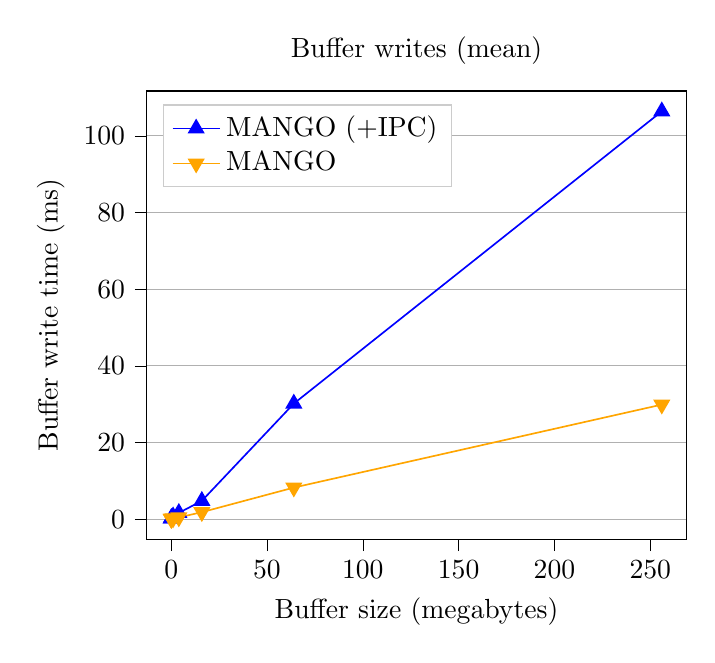
\begin{tikzpicture}

\definecolor{color0}{rgb}{1,0.647058823529412,0}

\begin{axis}[
legend cell align={left},
legend style={
  fill opacity=1,
  draw opacity=1,
  text opacity=1,
  at={(0.03,0.97)},
  anchor=north west,
  draw=white!80!black
},
tick align=outside,
tick pos=left,
title={Buffer writes (mean)},
x grid style={white!69.0196078431373!black},
xlabel={Buffer size (megabytes)},
xmin=-12.78359375, xmax=268.79921875,
xtick style={color=black},
y grid style={white!69.0196078431373!black},
ylabel={Buffer write time (ms)},
ymajorgrids,
ymin=-5.26581299425837, ymax=111.736714879426,
ytick style={color=black}
]
\addplot [semithick, blue, mark=triangle*, mark size=3, mark options={solid}]
table {%
0.015625 0.194150155778894
0.0625 0.185609424242424
0.25 0.288342966101695
1 0.705753933333333
4 1.615443825
16 4.75873836842105
64 30.1467156842105
256 106.418418157895
};
\addlegendentry{MANGO (+IPC)}
\addplot [semithick, color0, mark=triangle*, mark size=3, mark options={solid,rotate=180}]
table {%
0.015625 0.0711760703517588
0.0625 0.0524837272727273
0.25 0.0730327627118644
1 0.17710135
4 0.44483658974359
16 1.80250955
64 8.22336425
256 29.8767647
};
\addlegendentry{MANGO}
\end{axis}

\end{tikzpicture}

    } 
    }}%
    \qquad
    \subfloat[\centering Mean buffer read time]{{
        \resizebox{!}{160pt}{
            % This file was created by tikzplotlib v0.9.8.
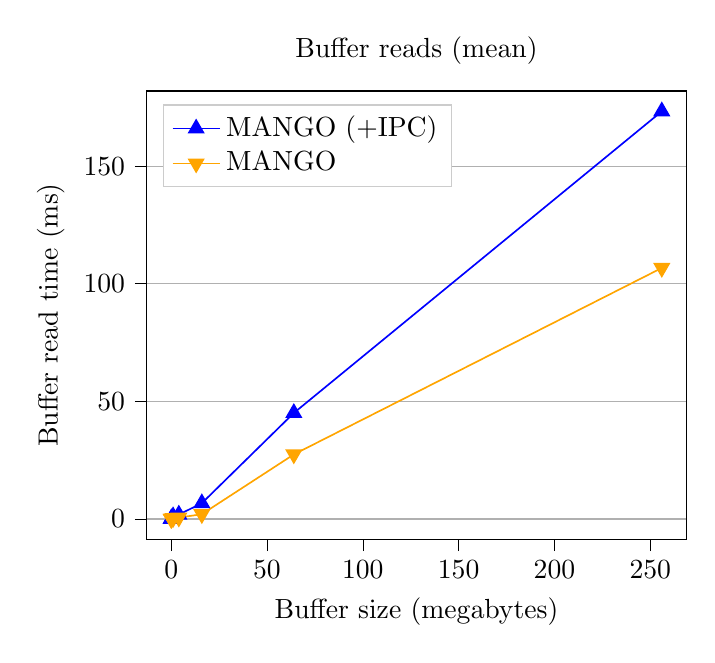
\begin{tikzpicture}

\definecolor{color0}{rgb}{1,0.647058823529412,0}

\begin{axis}[
legend cell align={left},
legend style={
  fill opacity=1,
  draw opacity=1,
  text opacity=1,
  at={(0.03,0.97)},
  anchor=north west,
  draw=white!80!black
},
tick align=outside,
tick pos=left,
title={Buffer reads (mean)},
x grid style={white!69.0196078431373!black},
xlabel={Buffer size (megabytes)},
xmin=-12.78359375, xmax=268.79921875,
xtick style={color=black},
y grid style={white!69.0196078431373!black},
ylabel={Buffer read time (ms)},
ymajorgrids,
ymin=-8.627191262, ymax=181.985046422,
ytick style={color=black}
]
\addplot [semithick, blue, mark=triangle*, mark size=3, mark options={solid}]
table {%
0.015625 0.0851318888888889
0.0625 0.12115998
0.25 0.293384266666667
1 1.14153996666667
4 1.86527426315789
16 6.7041604
64 45.0642416
256 173.3208538
};
\addlegendentry{MANGO (+IPC)}
\addplot [semithick, color0, mark=triangle*, mark size=3, mark options={solid,rotate=180}]
table {%
0.015625 0.03700136
0.0625 0.0445138367346939
0.25 0.100272066666667
1 0.3423668
4 0.580875789473684
16 2.02201494736842
64 27.4426727
256 106.7236178
};
\addlegendentry{MANGO}
\end{axis}

\end{tikzpicture}

        } 
    }}%
    \captionsetup{justification=centering}
    \caption{Mean buffer transfer times for HotSpot}%
    \label{fig:hotspot_buffer_transfers_mean_ipc}%
\end{figure}


\begin{figure}%
    \centering
    \subfloat[\centering Mean buffer write time]{{
        \resizebox{!}{160pt}{
        % This file was created by tikzplotlib v0.9.8.
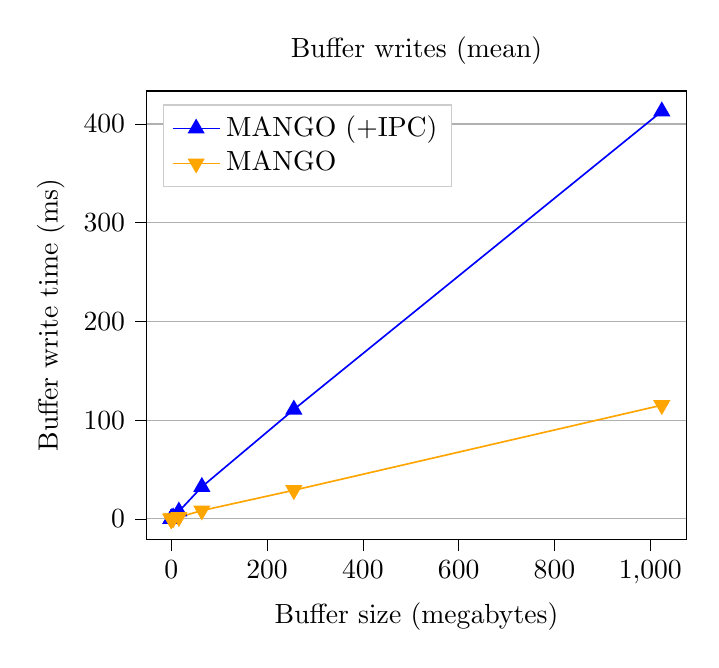
\begin{tikzpicture}

\definecolor{color0}{rgb}{1,0.647058823529412,0}

\begin{axis}[
legend cell align={left},
legend style={
  fill opacity=1,
  draw opacity=1,
  text opacity=1,
  at={(0.03,0.97)},
  anchor=north west,
  draw=white!80!black
},
tick align=outside,
tick pos=left,
title={Buffer writes (mean)},
x grid style={white!69.0196078431373!black},
xlabel={Buffer size (megabytes)},
xmin=-51.195849609375, xmax=1075.13432617188,
xtick style={color=black},
y grid style={white!69.0196078431373!black},
ylabel={Buffer write time (ms)},
ymajorgrids,
ymin=-20.58924334, ymax=433.44303294,
ytick style={color=black}
]
\addplot [semithick, blue, mark=triangle*, mark size=3, mark options={solid}]
table {%
0.0009765625 0.166594494949495
0.001953125 0.1613867
0.00390625 0.197607433333333
0.0078125 0.2003528
0.015625 0.14658275
0.03125 0.1526589
0.0625 0.1957964
0.2490234375 0.283896161616162
0.998046875 0.57725816
3.99609375 1.61366510344828
15.9921875 7.58525995
63.984375 32.5063535
255.96875 110.8095187
1023.9375 412.8052022
};
\addlegendentry{MANGO (+IPC)}
\addplot [semithick, color0, mark=triangle*, mark size=3, mark options={solid,rotate=180}]
table {%
0.0009765625 0.0549379696969697
0.001953125 0.05452808
0.00390625 0.0607788
0.0078125 0.06594505
0.015625 0.0485874
0.03125 0.0518924
0.0625 0.0560475
0.2490234375 0.0731669381443299
0.998046875 0.14242536
3.99609375 0.479685551724138
15.9921875 1.85305526315789
63.984375 8.46083815
255.96875 29.0700347
1023.9375 115.2031104
};
\addlegendentry{MANGO}
\end{axis}

\end{tikzpicture}

    } 
    }}%
    \qquad
    \subfloat[\centering Mean buffer read time]{{
        \resizebox{!}{160pt}{
            % This file was created by tikzplotlib v0.9.8.
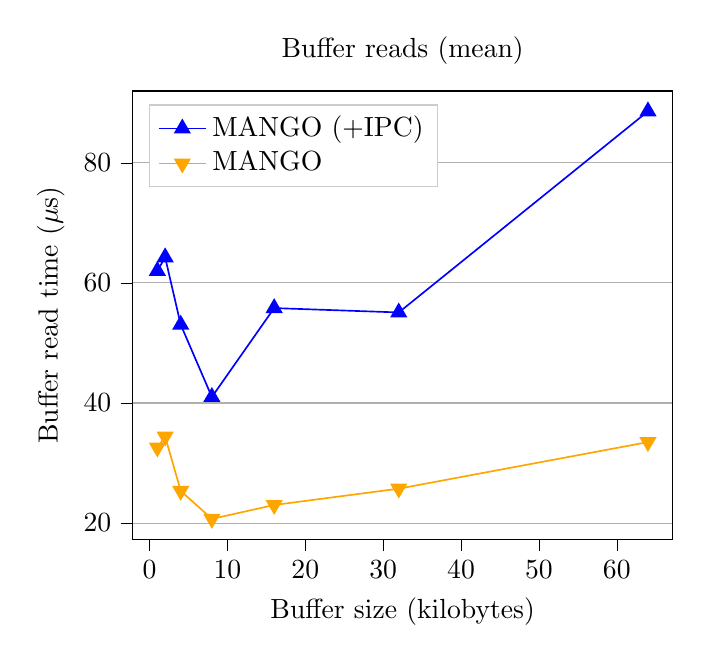
\begin{tikzpicture}

\definecolor{color0}{rgb}{1,0.647058823529412,0}

\begin{axis}[
legend cell align={left},
legend style={
  fill opacity=1,
  draw opacity=1,
  text opacity=1,
  at={(0.03,0.97)},
  anchor=north west,
  draw=white!80!black
},
tick align=outside,
tick pos=left,
title={Buffer reads (mean)},
x grid style={white!69.0196078431373!black},
xlabel={Buffer size (kilobytes)},
xmin=-2.15, xmax=67.15,
xtick style={color=black},
y grid style={white!69.0196078431373!black},
ylabel={Buffer read time ($\mu$s)},
ymajorgrids,
ymin=17.3005589473684, ymax=91.9736305263158,
ytick style={color=black}
]
\addplot [semithick, blue, mark=triangle*, mark size=3, mark options={solid}]
table {%
1 62.00486
2 64.2638979591837
4 53.0405666666667
8 41.00225
16 55.80855
32 55.0811
64 88.5794
};
\addlegendentry{MANGO (+IPC)}
\addplot [semithick, color0, mark=triangle*, mark size=3, mark options={solid,rotate=180}]
table {%
1 32.5831616161616
2 34.40658
4 25.3578666666667
8 20.6947894736842
16 23.0111052631579
32 25.7314
64 33.4862
};
\addlegendentry{MANGO}
\end{axis}

\end{tikzpicture}

        } 
    }}%
    \captionsetup{justification=centering}
    \caption{Mean buffer transfer times for PathFinder}%
    \label{fig:pathfinder_buffer_transfers_mean_ipc}%
\end{figure}

\subsection{Overall Performance Analysis}

At first glance, if we include the IPC overhead, our initial implementation of the HHAL and restructuring of the MANGO stack is certainly not competitive with state-of-the-art programming models such as CUDA and OpenCL. 

Communicating between multiple processes through sockets significantly reduces performance when working within the same cluster, as more efficient communication could be adopted. If the HHAL, Barbeque and the MANGO API host run on the same machine, all communication could be done through shared memory instead of a socket. In addition, kernel executions and buffer transfers could be done entirely through a library linked directly to the MANGO host, without the need of any IPC. Allowing the computer to work on in this sort of "hybrid" mode would let MANGO achieve throughput inline with the initial metrics we presented, which do not take into account IPC.

It is important to note however that some IPC will still be needed within the same computer, as both Barbeque and MANGO need access to the HHAL for different reasons. Barbeque needs to allocate and deallocate resources while MANGO needs to execute the kernels with these same allocated resources. As they do not co-exist in the same process (Barbeque always works as a daemon, which could be connected to more than just MANGO) and need to access the same HHAL information, it is a requirement for at least some bookkeeping of the HHAL to always exist as separate server.

Although this discussed approach works for a single cluster, it is not extensible to a distributed system. If the target device runs on a separate computer from the MANGO host, there is no shared memory available and no way to directly talk with the device through a simple library like it would be possible with the device physically attached to the host. 

For this reason, we first presented our measurements without taking into account IPC, as this is a fairer comparison between the different programming models. The CUDA and OpenCL implementations assume that the host will be connected directly to the accelerators, thus they do not need to implement any kind of external communication. However, once we introduce a second machine, the overhead will be similar, if not exactly the same, for any model used as coordination between the host and device across a distributed system will be a requirement.

By creating the HHAL in a client-server fashion we followed the approach used when creating the initial HN library, which allows the HHAL server to be easily distributed and run on a separate cluster. Once the platform matures, however, the improvements mentioned previously will be very important for the cases when the MANGO host and the HHAL do run on a single machine. This topic is discussed further in section \ref{sub-sect:hhal-hybrid-mode}.

Improvements can also be made on the HHAL side, without taking into account IPC. First, the overheads experienced for kernel executions can be attributed to the CUDA device context assignment which is currently repeated for each kernel launch. This is necessary, as we want MANGO to be able to run a kernel on any of the available GPUs. However, as the CUDA device context is set on a per-thread basis, this overhead could be avoided. In principle it would be possible to create a separate thread for each available device and assign a fixed context to each one as soon as the HHAL server is up and running.

Second, buffer transfers could be made asynchronous. By making the HHAL server multithreaded and enqueueing buffer transfers in different CUDA streams a bigger portion of the available PCI-E bandwidth could be exploited, as well as allowing for the ability to overlap data transfers and kernel executions as seen in \cite{overlap-data-transfers-cuda}.

\subsection{Programmability}

The results for the HotSpot benchmark can be seen in table \ref{tab:hotspot-loc} while the ones for PathFinder are in table \ref{tab:pathfinder-loc}.

\begin{table}
    \centering
    \begin{tabular}{l|c|c|c|c|c|c}
    \textit{Model} & \textit{Kernel (LOC)} & \textit{Kernel (RD)} & \textit{Host (LOC)} & \textit{Host (RD)} & \textit{Total (LOC)} & \textit{Total (RD)} \\ \hline
    MANGO & 84 & 0\% & 190 & 0\% & 274 & 0\% \\
    CUDA & 84 & 0\% & 166 & -13\% & 250 & -9\% \\
    OpenCL & 84 & 0\% & 212 & 12\% & 296 & 8\%  
    \end{tabular}
    \captionsetup{justification=centering}
    \caption{Lines of code for HotSpot benchmark}
    \label{tab:hotspot-loc}
\end{table}

\begin{table}
    \centering
    \begin{tabular}{l|c|c|c|c|c|c}
    \textit{Model} & \textit{Kernel (LOC)} & \textit{Kernel (RD)} & \textit{Host (LOC)} & \textit{Host (RD)} & \textit{Total (LOC)} & \textit{Total (RD)} \\ \hline
    MANGO & 59 & 0\% & 133 & 0\% & 192 & 0\% \\
    CUDA & 59 & 0\% & 108 & -19\% & 167 & -13\% \\
    OpenCL & 59 & 0\% & 188 & 41\% & 247 & 29\%  
    \end{tabular}
    \captionsetup{justification=centering}
    \caption{Lines of code for PathFinder benchmark}
    \label{tab:pathfinder-loc}
\end{table}

When comparing kernel LOC we can see that they are equal across all implementations of the same benchmark. As MANGO uses the same kernel code as the CUDA implementation, this is expected. In the case of OpenCL, its kernels are also optimized for GPU execution and thus follow the same access pattern as a CUDA kernel. The only differences among the kernels being CUDA and OpenCL specific keywords and functions, which have a 1-to-1 mapping between each other.

On the host side, the CUDA implementation gains the upper hand on MANGO, needing 9\% less code for HotSpot and 13\% less code for PathFinder. On the other hand OpenCL requires 8\% and 29\% more code for each respective benchmark. These differences are mostly related to the following factors:

\textbf{Kernel function calls:} the single source nature of CUDA code allows these implementations to call a kernel like any other function. Meanwhile MANGO requires creating multiple argument objects, one for each of the kernel inputs and grouping them into a \texttt{KernelArguments} object to be able to start the kernel execution. OpenCL faces a similar issue as it also needs explicit \texttt{setKernelArg} calls for each kernel input. This gives a big advantage to CUDA, with MANGO and OpenCL being very similar to each other.

\textbf{Kernel loading:} both MANGO and OpenCL need to load kernel code from an external file. For MANGO this only requires creating a \texttt{KernelFunction} object, loading a file (single call to the \texttt{load} function of a \texttt{KernelFunction}) and registering the kernel to the \texttt{Context}. Meanwhile OpenCL requests that the kernel code is provided as a C string, leaving the file loading code to the user, who also needs to make function calls to build the program and create a kernel object. The CUDA implementation is not required to do any of the previous work, as the kernel code can be called directly and is compiled along with the host code.

\textbf{Resource deallocations:} while all programming models need to explicitly request resource allocation for input and output buffers, MANGO does not leave the user with the responsibility to perform the inverse operations, at least not individually. When the MANGO implementations finish, they can simply call the context deallocation function and all requested resources will be correctly released. On the other hand, both OpenCL and CUDA require explicit release of resources. In the case of CUDA, this only entails calling \texttt{cudaFree} for each \texttt{cudaMalloc} call, for OpenCL it is much more involved, however. The programmer needs to release, on top of the allocated buffers, the following resources: \texttt{CommandQueue}, \texttt{Kernel}, \texttt{Program}, \texttt{Context}, a buffer for the program source string, a buffer for querying device ids and a buffer for querying platform ids.

\textbf{Device selection:} OpenCL requires manual querying of the available platforms on the host as well as the available devices in order to select the device to use for the benchmark. Both are multi-step processes requiring multiple function calls and host heap memory allocations. As CUDA only runs on Nvidia GPUs, one only needs to select a particular device ID among the ones available, but that can also be skipped (and was, for our tests) if there is only a single GPU available or there is no preference in which GPU to run the kernel. Finally, MANGO does all this work automatically, needing no input from the user apart from providing the device kernels along with information about which platform they target (in this case Nvidia). In the background, BBQUE and the HHAL will make sure to assign the kernel to run on the most suitable device. This approach is significantly more optimal in terms of resource management, at no extra code cost for the MANGO user. Neither CUDA nor OpenCL provide similar functionalities, so an equivalent implementation would require considerably more programmer effort.

\textbf{Error handling:} as both CUDA and OpenCL work with exit codes in order to communicate runtime errors, there is a need to perform explicit error handling at each function call in their benchmark implementations. For brevity, most of this error handling was extracted into preprocessor macros, so they do not contribute significantly to the total LOC. Some OpenCL calls however cannot be easily handled by a macro and need extra error handling code. Meanwhile, the last layer of the MANGO API maps runtime errors into exceptions so they can be handled more easily by the user. Note that the error handling code added for both CUDA and OpenCL follows a "fail-fast" approach, essentially converting an error code coming from the library into a program crash, similar to throwing an exception, like MANGO does.

A breakdown of LOC differences for these particular sections of the code in both benchmarks can be seen in tables \ref{tab:hotspot-factors-loc} and \ref{tab:pathfinder-factors-loc} which refer to HotSpot and PathFinder respectively. As shown here, the main disadvantage of MANGO over CUDA is due to the kernel call code. This could be improved by leveraging C++'s templates, allowing for a variety of argument types and quantities to be supplied directly to MANGO's \texttt{kernel\_launch} call. This will turn the implementation of the function significantly more complex, but will provide a much more concise API for the users of the platform.

\begin{table}
    \centering
    \begin{tabular}{l|c|c|c|c|c|c}
    \textit{Model} & \textit{Kernel call} & \textit{Kernel load} & \textit{Deallocations} & \textit{Device select} & \textit{Error handling} & \textit{Total} \\ \hline
    MANGO & 20 & 3 & 1 & 0 & 0 & 24 \\
    CUDA & 7 & 0 & 3 & 0 & 7 & 17 \\
    OpenCL & 16 & 16 & 10 & 14 & 14 & 70  
    \end{tabular}
    \captionsetup{justification=centering}
    \caption{Size of relevant sections of code in HotSpot benchmark}
    \label{tab:hotspot-factors-loc}
\end{table}

\begin{table}
    \centering
    \begin{tabular}{l|c|c|c|c|c|c}
    \textit{Model} & \textit{Kernel call} & \textit{Kernel load} & \textit{Deallocations} & \textit{Device select} & \textit{Error handling} & \textit{Total} \\ \hline
    MANGO & 15 & 3 & 1 & 0 & 0 & 19 \\
    CUDA & 6 & 0 & 3 & 0 & 7 & 16 \\
    OpenCL & 11 & 16 & 10 & 14 & 14 & 65  
    \end{tabular}
    \captionsetup{justification=centering}
    \caption{Size of relevant sections of code in PathFinder benchmark}
    \label{tab:pathfinder-factors-loc}
\end{table}

